\documentclass[journal]{IEEEtran}
\usepackage{amsmath,amsfonts}
\usepackage{algpseudocode}
\usepackage{algorithm}
\usepackage{array}
\usepackage{booktabs}
\usepackage[caption=false,font=normalsize,labelfont=sf,textfont=sf]{subfig}
\usepackage{multirow}
\usepackage{siunitx}
\usepackage{textcomp}
\usepackage{stfloats}
\usepackage{threeparttable}
\usepackage{url}
\usepackage{verbatim}
\usepackage{graphicx}
\usepackage{tikz}
\usepackage{cite}
\usetikzlibrary{positioning,calc}
\hyphenation{op-tical net-works semi-conduc-tor IEEE-Xplore}
\usepackage[american]{circuitikz}
\usetikzlibrary{calc, positioning, arrows.meta}
\hbadness=10000
\vbadness=10000
\hfuzz=8pt
\newcommand{\compactpartial}[2]{%
    \compactpartialaux#1\compactstop#2\compactstop}
\def\compactpartialaux\partial#1\compactstop\partial#2\compactstop{%
    \partial_{#2}#1}
% updated with editorial comments 8/9/2021

\begin{document}

\title{Optimal Control of Static Var Compensators for Power Quality Enhancement in Three-Phase Distribution Systems}

\author{IEEE Publication Technology,~\IEEEmembership{Staff,~IEEE,}
        % <-this % stops a space
\thanks{This paper was produced by the IEEE Publication Technology Group. They are in Piscataway, NJ.}% <-this % stops a space
\thanks{Manuscript received April 19, 2021; revised August 16, 2021.}}

% The paper headers
\markboth{Journal of \LaTeX\ Class Files,~Vol.~14, No.~8, August~2021}%
{Shell \MakeLowercase{\textit{et al.}}: A Sample Article Using IEEEtran.cls for IEEE Journals}

\IEEEpubid{}
% Remember, if you use this you must call \IEEEpubidadjcol in the second
% column for its text to clear the IEEEpubid mark.

\maketitle

\begin{abstract}
This paper proposes a nonlinear optimization methodology for the control of static var compensators (SVCs) in three-phase distribution systems. The proposed approach is formulated based on the equations of the Harmonic Three-Phase Current Injection Method (MICTH) and represents each compensator through its topology-dependent harmonic current-injection equations and admissible control variables. Consequently, the framework can be adapted to wye- or delta-connected SVCs and to different internal arrangements, provided that their electrical models and operating limits are available. The numerical implementation adopts delta-connected fixed-capacitor--thyristor-controlled-reactor (FC--TCR) compensators and independently adjusts the firing angle of each branch, allowing branch-dependent reactive-power injection according to the operating condition of the network. In addition to voltage and THD constraints, the formulation includes a voltage unbalance factor (VUF) constraint computed from positive- and negative-sequence voltage components, while the objective function combines voltage-deviation, negative-sequence, and phase-imbalance indices. The methodology is evaluated in the IEEE 33-bus distribution system under balanced and unbalanced loading conditions. Results indicate that the proposed strategy increases the loading capability of the controlled buses, improves voltage profiles, and, in appropriate operating conditions, contributes to the reduction of phase unbalance without violating the prescribed THD limits. These results demonstrate the potential of optimized SVC control as a flexible alternative for enhancing power quality of distribution systems under demanding loading scenarios.
\end{abstract}

\begin{IEEEkeywords}
Three-phase distribution systems, static var compensators, nonlinear optimization, power quality, harmonic distortion.
\end{IEEEkeywords}

\section{Introduction}
\IEEEPARstart{D}{istribution} systems operate under increasingly complex technical conditions due to the combined effects of load variability, phase unbalance, nonlinear consumer devices, and the limited voltage support typically available along radial feeders. In practical networks, these characteristics may lead to unequal phase loading, harmonic distortion, voltage drop at remote buses, and reduced operating margins, especially in long feeders and under loading levels above nominal conditions~\cite{loji2023operational}. From the operational viewpoint, these challenges are further intensified by the ongoing transformation of distribution grids, particularly with the increasing penetration of distributed generation and the rapid growth of electric-vehicle charging demand~\cite{nasir2024hosting,ghaffari2025planning}. In parallel, artificial-intelligence techniques are increasingly being investigated for the detection, classification, prediction, and mitigation of power-quality disturbances in distribution systems~\cite{dehaghani2025ai}.

Within this scenario, power-electronics-based equipment has become increasingly relevant in distribution systems because it enables faster and more flexible actions for voltage regulation, reactive power compensation, power-flow support, and broader power-quality improvement~\cite{Stanelyte2020VoltVar}. This aspect is particularly important because voltage drop at the end of feeders and phase unbalance remain among the most persistent problems in distribution operation, while conventional utility assets still offer limited dynamic controllability in many practical networks. In other words, distribution companies often need to operate systems whose monitoring and control capabilities are still insufficient for real-time mitigation of local disturbances and phase-dependent voltage deviations, especially in low-observability feeders~\cite{Yadav2023DSSE}. Among the available solutions, static var compensators composed of fixed capacitors and thyristor-controlled reactors have attracted attention because they allow continuous reactive-power control and are employed in voltage-regulation and reactive-power compensation applications~\cite{Stanelyte2020VoltVar,Liu2020SVCUnbalance}.

However, voltage regulation alone may be insufficient when the problem is analyzed from a power-quality perspective. Power-electronic compensators are nonlinear devices and may inject harmonic components into the network; in thyristor-based compensators, characteristic low-order harmonics such as the 5th, 7th, 11th, and 13th are commonly discussed, depending on the circuit configuration and filtering conditions~\cite{Kraimia2021SVCHarmonics,Zheng2021SVCHarmonicFailure}. In addition, fixed capacitors may interact with the inductive elements of the network and create resonance conditions capable of amplifying voltage distortion, increasing total harmonic distortion (THD), and even contributing to overvoltage phenomena~\cite{Farzin2022CapacitorResonance}. Phase unbalance is also a critical issue because it may increase neutral currents, intensify losses and heating in conductors and equipment, and degrade the operating conditions of sensitive loads and rotating machines~\cite{Liu2020SVCUnbalance}. Therefore, voltage support, harmonic distortion, and phase unbalance should be addressed in an integrated way rather than as isolated phenomena.

In this context, the objective of this paper is to propose a nonlinear optimization methodology for the control of SVCs based on the Harmonic Three-Phase Current Injection Method (MICTH). MICTH is the harmonic extension of the Three-Phase Current Injection Method (TCIM) proposed for fundamental-frequency unbalanced power-flow calculations~\cite{garcia2000three,Arruda2003}. At the optimization level, the methodology is not restricted to a specific connection or internal SVC arrangement. Wye- and delta-connected devices, including common FC--TCR and TSC--TCR realizations and combinations of controlled or switched reactor and capacitor banks, can be represented by adapting the device current-injection equations, control variables, and operating limits~\cite{MathurVarma2002,IEEE1031_2011}. The numerical study specializes this general framework to a delta-connected FC--TCR SVC with independently controlled branches. This configuration was selected for the adopted three-wire system because direct control of the line-to-line branch susceptances provides effective negative-sequence compensation~\cite{Chen1999SVCBalance}; its harmonic behavior is examined in Section~\ref{subsec:svc_harmonics}. The formulation is structured to preserve acceptable voltage levels and explicitly enforce THD and voltage-unbalance limits, while voltage regulation, negative-sequence mitigation, and phase-magnitude balancing are handled directly in the objective function. The proposed approach is evaluated in the IEEE 33-bus distribution system~\cite{dolatabadi2021}, providing a computational framework for investigating the coordinated effects of nonlinear compensation, voltage support, harmonic performance, and phase balancing under different loading conditions.


% =========================================================================
% METHODOLOGY SECTION — IEEE/Elsevier compatible LaTeX
% Topic: Harmonic Power Flow with Multidimensional SVC Control Optimization
% =========================================================================

\section{Methodology}
\label{sec:methodology}

The methodology is presented in the order in which each operating point is
constructed and solved. First, the selected FC--TCR SVC and its harmonic
current injections are modeled. The resulting device model is then embedded
in the Harmonic Three-Phase Current Injection Method (MICTH), an extension of
the Three-Phase Current Injection Method (TCIM)~\cite{garcia2000three,Arruda2003}.
Next, the phase-dependent load trajectory and the reduced-space optimization
problem are defined. Finally, the SQP solver and the sequential solution
procedure are described.

% -------------------------------------------------------------------------
\subsection{Static Var Compensator Model}
\label{subsec:svc_rating}

In the proposed framework, the SVC installed at bus $k$ is represented at
harmonic order $h$ by the generic current-injection map

\begin{equation}
    \mathbf{I}^{(h)}_{\mathrm{SVC},k} =
    \mathbf{f}^{(h)}_{\mathrm{SVC},k}
    \!\left(\mathbf{V}_k,\mathbf{u}_k,\mathbf{p}_k\right),
    \label{eq:generic_svc_current}
\end{equation}

\noindent where $\mathbf{u}_k$ contains the controllable quantities and
$\mathbf{p}_k$ contains the electrical and connection parameters. Depending on
the SVC arrangement, $\mathbf{u}_k$ may include firing angles, equivalent
susceptance setpoints, or switching states. Therefore, the MICTH and
optimization layers require only the corresponding current injections,
sensitivities, and admissible control set; the incidence relations and device
equations may be replaced without changing the overall methodology. This
interface permits wye- or delta-connected implementations and different
combinations of TCR, thyristor-switched reactor (TSR), thyristor-switched
capacitor (TSC), fixed-capacitor, and filter
branches~\cite{MathurVarma2002,IEEE1031_2011}.
Discrete switching arrangements require the control variables and optimization
solver to be adapted accordingly, while the harmonic power-flow interface is
preserved.

For the numerical assessment, the generic representation in
\eqref{eq:generic_svc_current} is specialized to the frequency-domain FC--TCR
model described in~\cite{MathurVarma2002,Arruda2003}. The device is composed
of a linear fixed capacitor bank in parallel with a nonlinear TCR. Thus, its
nodal current is obtained from

\begin{equation}
    \mathbf{I}^{(h)}_{\mathrm{SVC},k} =
    \mathbf{I}^{(h)}_{\mathrm{TCR},k} +
    \mathbf{I}^{(h)}_{C,k},
    \label{eq:svc_current}
\end{equation}

Equation~\eqref{eq:svc_current} separates the linear capacitor branch, which
is directly included in
the harmonic admittance matrix, whereas the TCR branch is represented by a
controlled current injection whose Fourier components depend on the bus
voltage waveform and on the branch firing angle $\alpha_{j,\ell}$. This formulation is
appropriate for harmonic power-flow studies because the thyristor reactor
introduces coupling among harmonic frequencies, while the fixed capacitor
contributes a frequency-dependent susceptance that may affect both reactive
support and harmonic resonance conditions.

The delta connection is a choice of the numerical implementation rather than a
restriction of the methodology. It is preferred in the adopted three-wire
feeder because independently controlling the $ab$, $bc$, and $ca$ line-to-line
susceptances provides an effective mechanism for synthesizing a compensating
negative-sequence current~\cite{Chen1999SVCBalance}. A wye-connected SVC can be
included through the same generic map by replacing the connection incidence
matrix, phase-voltage relations, and rating equations. For the selected delta
case, equal branch susceptances reproduce conventional balanced reactive-power
support, whereas unequal susceptances enable phase-balancing control. The
triplen-harmonic property of balanced operation is derived separately in
Section~\ref{subsec:svc_harmonics}. The adopted notation for the selected
FC--TCR compensator is summarized in
Fig.~\ref{fig:delta_fc_tcr_svc}.

\begin{figure}[!t]
    \centering
\resizebox{\columnwidth}{!}{%
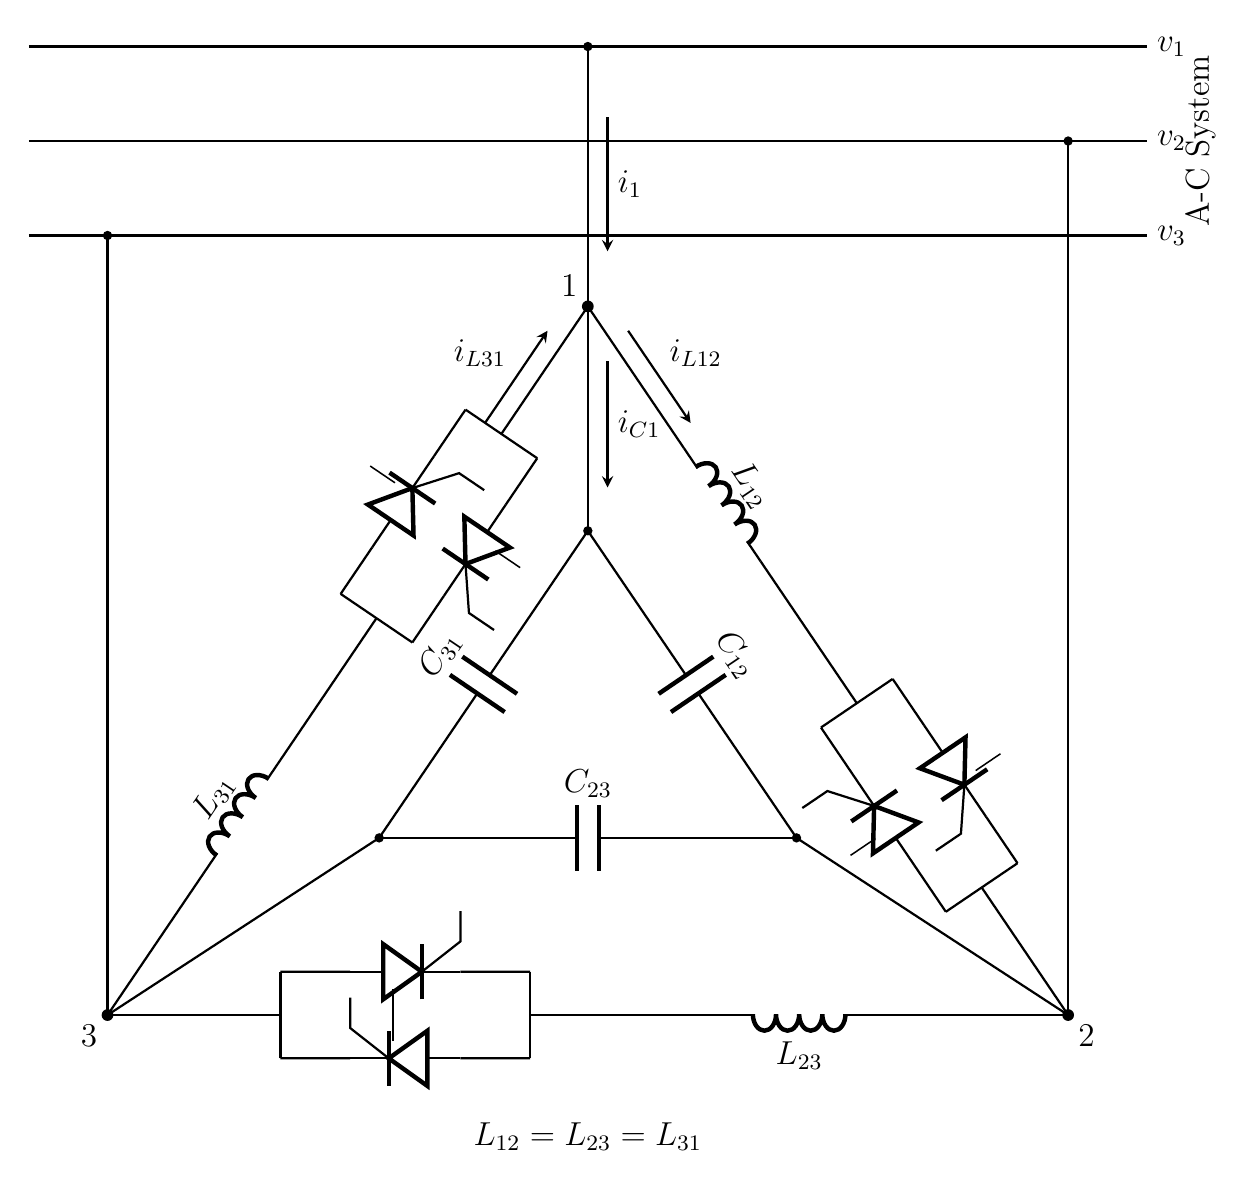
\begin{tikzpicture}[line width=0.8pt, every node/.style={font=\large}]

    % ==========================================
    % MACRO PARA O RAMO TCR (Indutor + Tiristores)
    % ==========================================
    % Desenha um indutor em série com um bloco de tiristores em antiparalelo.
    % #1: Nó inicial, #2: Nó final, #3: Label do indutor
    \newcommand{\drawTCR}[4]{
        % Coordenadas proporcionais ao longo do caminho
        \path (#1) -- (#2)
            coordinate[pos=0.20] (p1)
            coordinate[pos=0.36] (p2)
            coordinate[pos=0.56] (p3)
            coordinate[pos=0.82] (p4);

        % Fio inicial e indutor
        \draw (#1) -- (p1);
        \draw (p1) to[L, l=#3] (p2);
        \draw (p2) -- (p3);

        % Bloco de tiristores em antiparalelo, afastado do fio principal
        \coordinate (v_up) at ($(p3)!0.55cm!90:(p4)$);
        \coordinate (u_up) at ($(p4)!0.55cm!-90:(p3)$);
        \coordinate (v_dn) at ($(p3)!0.55cm!-90:(p4)$);
        \coordinate (u_dn) at ($(p4)!0.55cm!90:(p3)$);
        \coordinate (g_up) at ($(v_up)!0.55!(u_up)$);
        \coordinate (g_dn) at ($(v_dn)!0.55!(u_dn)$);

        \draw (p3) -- (v_up);
        \draw (p3) -- (v_dn);
        \draw (u_up) -- (p4);
        \draw (u_dn) -- (p4);
        \draw (v_up) to[Ty, mirror] (u_up);
        \draw (u_dn) to[Ty] (v_dn);

        % Gates destacados para fora do ramo, sem encostar no fio principal
        \draw[line width=0.55pt] ($(g_up)!0.22cm!#4:(u_up)$) -- ($(g_up)!0.60cm!#4:(u_up)$);
        \draw[line width=0.55pt] ($(g_dn)!0.22cm!#4:(v_dn)$) -- ($(g_dn)!0.60cm!#4:(v_dn)$);

        % Fio final
        \draw (p4) -- (#2);
    }

    % ==========================================
    % MACRO PARA SETAS DE CORRENTE PARALELAS
    % ==========================================
    \newcommand{\pararrow}[5]{
        \path (#1) -- (#2) coordinate[pos=#3] (as) coordinate[pos=#4] (ae);
        \coordinate (aso) at ($(as)!0.25cm!90:(#2)$);
        \coordinate (aeo) at ($(ae)!0.25cm!90:(#2)$);
        \draw[->, >=stealth] (aso) -- (aeo) node[midway, auto] {#5};
    }

    % ==========================================
    % COORDENADAS PRINCIPAIS DO SISTEMA
    % ==========================================
    % Vértices do Delta Externo
    \coordinate (N1) at (0, 3.3);
    \coordinate (N2) at (6.1, -5.7);
    \coordinate (N3) at (-6.1, -5.7);

    % Vértices do Delta Interno (Capacitores)
    \coordinate (J1) at (0, 0.45);
    \coordinate (J2) at (2.65, -3.45);
    \coordinate (J3) at (-2.65, -3.45);

    % ==========================================
    % SISTEMA A-C SUPERIOR E CONEXÕES
    % ==========================================
    \draw (-7.1, 6.6) -- (7.1, 6.6) node[right] {$v_1$};
    \draw (-7.1, 5.4) -- (7.1, 5.4) node[right] {$v_2$};
    \draw (-7.1, 4.2) -- (7.1, 4.2) node[right] {$v_3$};
    \node[rotate=90, anchor=south] at (8.1, 5.4) {A-C System};

    % Ligações dos nós principais às linhas A-C com nós (bolinhas)
    \draw (N1) -- (0, 6.6) node[circle,fill,inner sep=1.2pt, font=\normalsize]{};
    \draw (N2) -- (6.1, 5.4) node[circle,fill,inner sep=1.2pt, font=\normalsize]{};
    \draw (N3) -- (-6.1, 4.2) node[circle,fill,inner sep=1.2pt, font=\normalsize]{};

    % ==========================================
    % DELTA EXTERNO (TCR)
    % ==========================================
    % Desenhando os 3 ramos usando a macro criada
    \drawTCR{N1}{N2}{$L_{12}$}{90}
    \drawTCR{N2}{N3}{$L_{23}$}{-90}
    \drawTCR{N3}{N1}{$L_{31}$}{90}

    % ==========================================
    % DELTA INTERNO (Fixed Capacitors)
    % ==========================================
    % Conexões dos vértices externos para os vértices internos
    \draw (N1) -- (J1);
    \draw (N2) -- (J2);
    \draw (N3) -- (J3);

    % Pontos (bolinhas) no delta interno
    \node[circle, fill=black, inner sep=1.2pt, font=\normalsize] at (J1) {};
    \node[circle, fill=black, inner sep=1.2pt, font=\normalsize] at (J2) {};
    \node[circle, fill=black, inner sep=1.2pt, font=\normalsize] at (J3) {};

    % Ramos dos Capacitores
    \draw (J1) to[C, l=$C_{12}$] (J2);
    \draw (J2) to[C, l_=$C_{23}$] (J3); % l_ inverte o lado do texto
    \draw (J3) to[C, l=$C_{31}$] (J1);

    % ==========================================
    % RÓTULOS E CORRENTES
    % ==========================================
    % Numeração dos nós
    \node[circle, fill=black, inner sep=1.5pt, font=\normalsize] at (N1) {};
    \node[above left] at (N1) {1};
    
    \node[circle, fill=black, inner sep=1.5pt, font=\normalsize] at (N2) {};
    \node[below right] at (N2) {2};
    
    \node[circle, fill=black, inner sep=1.5pt, font=\normalsize] at (N3) {};
    \node[below left] at (N3) {3};

    % Setas de corrente manuais
    \draw[->, >=stealth] (0.25, 5.7) -- (0.25, 4.0) node[midway, right] {$i_1$};
    \draw[->, >=stealth] (0.25, 2.6) -- (0.25, 1.0) node[midway, right] {$i_{C1}$};

    % Setas de corrente nos ramos do delta usando a macro paralela
    \pararrow{N1}{N2}{0.05}{0.18}{$i_{L12}$}
    \pararrow{N3}{N1}{0.82}{0.95}{$i_{L31}$}

    % ==========================================
    % EQUAÇÃO INFERIOR
    % ==========================================
    \node at (0, -7.25) {$L_{12} = L_{23} = L_{31}$};

\end{tikzpicture}%
}
    \caption{Delta-connected FC--TCR SVC installed at bus $j$ using the
    branch notation adopted in the proposed formulation. Each delta branch
    $\ell\in\{ab,bc,ca\}$ contains a fixed capacitor $C_{j,\ell}$ in parallel
    with a TCR branch controlled by the firing angle $\alpha_{j,\ell}$.}
    \label{fig:delta_fc_tcr_svc}
\end{figure}

At the fundamental frequency, the equivalent branch susceptance of SVC $j$ in
branch $\ell \in \{ab,bc,ca\}$ is written as~\cite{MathurVarma2002}

\begin{equation}
    B_{\mathrm{SVC},j,\ell}(\alpha_{j,\ell}) =
    B_{C,j,\ell} - B_{\mathrm{TCR},j,\ell}(\alpha_{j,\ell}),
    \label{eq:svc_susceptance}
\end{equation}

\noindent in which $B_{C,j,\ell}$ is the fixed-capacitor susceptance and
$B_{\mathrm{TCR},j,\ell}(\alpha_{j,\ell})$ is the controllable reactor
susceptance of the corresponding delta branch. For a delta-connected device,
each branch is subjected to the line-to-line voltage. Therefore, for a system
with nominal line-to-line voltage $V_{\mathrm{LL,nom}}$, the corresponding
reactive-power rating is computed as

\begin{equation}
    Q_{\mathrm{SVC},j} = V_{\mathrm{LL,nom}}^2
    \sum_{\ell \in \{ab,bc,ca\}} \left|B_{\mathrm{SVC},j,\ell}\right|,
    \label{eq:svc_rating}
\end{equation}

In~\eqref{eq:svc_rating}, $V_{\mathrm{LL,nom}}$ is expressed in kV,
$B_{\mathrm{SVC},j,\ell}$ in siemens, and $Q_{\mathrm{SVC},j}$ in MVAr. Since
an SVC is a predominantly reactive
shunt compensator, its apparent-power rating is taken as
$S_{\mathrm{SVC},j} \approx |Q_{\mathrm{SVC},j}|$. The electrical
parameters and reactive-power operating ranges adopted for the numerical
assessment are reported in Section~\ref{sec:results}.

% -------------------------------------------------------------------------
\subsection{Harmonic Effects of the Selected Delta SVC}
\label{subsec:svc_harmonics}

For the selected delta-connected FC--TCR implementation, the harmonic currents
depend not only on the firing-angle value, but also on whether the three
branches are operated symmetrically. For each branch
$\ell\in\{ab,bc,ca\}$, the TCR current can be
expanded in a Fourier series, following the standard mathematical foundation of
harmonic analysis and the electrical formulation of the TCR
current~\cite{katznelson2004introduction,MathurVarma2002}, as

\begin{equation}
    i_{j,\ell}(t)=\sum_{h\in\mathcal{H}}
    I_{j,\ell}^{(h)}(\alpha_{j,\ell})
    \cos\!\big(h\omega t+\varphi_{j,\ell}^{(h)}\big),
    \label{eq:tcr_branch_fourier}
\end{equation}

In~\eqref{eq:tcr_branch_fourier}, the harmonic magnitude
$I_{j,\ell}^{(h)}$ and phase
$\varphi_{j,\ell}^{(h)}$ are functions of the firing angle and of the
line-to-line voltage applied to that branch. The harmonic current injected
into the feeder phases is obtained from the delta incidence relation

\begin{equation}
    \begin{bmatrix}
    I_{j,a}^{(h)} \\
    I_{j,b}^{(h)} \\
    I_{j,c}^{(h)}
    \end{bmatrix}
    =
    \begin{bmatrix}
    1 & 0 & -1 \\
    -1 & 1 & 0 \\
    0 & -1 & 1
    \end{bmatrix}
    \begin{bmatrix}
    I_{j,ab}^{(h)} \\
    I_{j,bc}^{(h)} \\
    I_{j,ca}^{(h)}
    \end{bmatrix},
    \label{eq:delta_harmonic_currents}
\end{equation}

\noindent which shows that the harmonic current of each phase is the
difference between two adjacent delta-branch harmonic currents.

If the SVC is balanced, the three branches have equal parameters and equal
firing angles, i.e.,
$\alpha_{j,ab}=\alpha_{j,bc}=\alpha_{j,ca}=\alpha_j$. For balanced
line-to-line voltages, the branch harmonic phasors have equal magnitudes and
are phase-shifted by the harmonic order, so they can be written as

\begin{equation}
    \begin{bmatrix}
    I_{j,ab}^{(h)} \\
    I_{j,bc}^{(h)} \\
    I_{j,ca}^{(h)}
    \end{bmatrix}
    = I_j^{(h)}(\alpha_j)
    \begin{bmatrix}
    1 \\
    a^{-h} \\
    a^{h}
    \end{bmatrix},
    \qquad a=e^{j2\pi/3}.
    \label{eq:balanced_branch_harmonics}
\end{equation}

\noindent Substituting~\eqref{eq:balanced_branch_harmonics}
into~\eqref{eq:delta_harmonic_currents} gives the line-current harmonic
phasors

\begin{equation}
    \begin{bmatrix}
    I_{j,a}^{(h)} \\
    I_{j,b}^{(h)} \\
    I_{j,c}^{(h)}
    \end{bmatrix}
    = I_j^{(h)}(\alpha_j)
    \begin{bmatrix}
    1-a^{h} \\
    a^{-h}-1 \\
    a^{h}-a^{-h}
    \end{bmatrix}.
    \label{eq:balanced_delta_line_harmonics}
\end{equation}

\noindent Equation~\eqref{eq:balanced_delta_line_harmonics} makes the
harmonic cancellation in a balanced delta explicit~\cite{MathurVarma2002}.
If $h=3m$, then
$a^h=a^{-h}=1$, and therefore

\begin{equation}
    I_{j,a}^{(h)}=I_{j,b}^{(h)}=I_{j,c}^{(h)}=0,
    \qquad h=3m.
    \label{eq:triplen_delta_cancellation}
\end{equation}

\noindent Thus, triplen harmonics such as the 3rd, 9th, and 15th may exist as
branch currents inside the closed delta, but they are ideally not injected
into the feeder line currents. For non-triplen orders, the factor in
\eqref{eq:balanced_delta_line_harmonics} is not zero, and the SVC injects a
balanced set of line-current harmonics into the network. These injected
harmonics keep a definite sequence: orders $h=3m+1$ form a positive-sequence
set, whereas orders $h=3m-1$ form a negative-sequence set. Since the ideal TCR
waveform has half-wave symmetry, even harmonics are not produced under
balanced conditions; therefore, the main harmonic currents injected by a
balanced delta SVC are the non-triplen odd orders, typically the 5th, 7th,
11th, 13th, and higher orders, in addition to the fundamental reactive
current. Hence, balanced operation does not mean that no harmonics are
injected into the system; it means that the injected harmonics are balanced
non-triplen components, while the triplen components remain confined to the
delta branch currents under ideal symmetry.

If the firing angles are not balanced, the branch harmonic phasors can no
longer be represented by a single magnitude $I_j^{(h)}(\alpha_j)$ and fixed
phase shifts. Instead,

\begin{equation}
    \begin{bmatrix}
    I_{j,ab}^{(h)} \\
    I_{j,bc}^{(h)} \\
    I_{j,ca}^{(h)}
    \end{bmatrix}
    =
    \begin{bmatrix}
    I_{j,ab}^{(h)}(\alpha_{j,ab}) \\
    I_{j,bc}^{(h)}(\alpha_{j,bc}) \\
    I_{j,ca}^{(h)}(\alpha_{j,ca})
    \end{bmatrix},
    \label{eq:unbalanced_branch_harmonics}
\end{equation}

\noindent and the resulting phase currents must be decomposed into sequence
components at each harmonic order as

\begin{equation}
    \begin{bmatrix}
    I_{j,0}^{(h)} \\
    I_{j,+}^{(h)} \\
    I_{j,-}^{(h)}
    \end{bmatrix}
    =\frac{1}{3}
    \begin{bmatrix}
    1 & 1 & 1 \\
    1 & a^{h} & a^{2h} \\
    1 & a^{2h} & a^{h}
    \end{bmatrix}
    \begin{bmatrix}
    I_{j,a}^{(h)} \\
    I_{j,b}^{(h)} \\
    I_{j,c}^{(h)}
    \end{bmatrix}.
    \label{eq:harmonic_sequence_decomposition}
\end{equation}

\noindent In this case, unequal firing angles intentionally produce
fundamental-frequency asymmetry that can compensate the negative-sequence
voltage created by unbalanced loads. However, the same branch-dependent
conduction also changes the harmonic magnitudes and phases in
\eqref{eq:unbalanced_branch_harmonics}, so additional positive- and
negative-sequence harmonic components may appear in
\eqref{eq:harmonic_sequence_decomposition}. For this reason, the proposed
optimization does not treat phase balancing and harmonic performance
independently: the firing angles are selected while explicitly constraining
THD$_V$, so that the harmonic distortion introduced by unbalanced branch-wise
control remains within the admissible limits.

% -------------------------------------------------------------------------
\subsection{Three-Phase Harmonic Power Flow}
\label{subsec:hpf}

The steady-state solution at each operating point is obtained with the
Harmonic Three-Phase Current Injection Method (MICTH), from the Portuguese
expression \textit{M\'etodo de Inje\c{c}\~ao de Correntes Trif\'asico
Harm\^onico}~\cite{Arruda2003}. MICTH extends the fundamental-frequency TCIM
in~\cite{garcia2000three} by solving the current mismatches of all phases and
harmonic orders in one rectangular-coordinate system. Linear network elements
are assembled in harmonic admittance matrices, whereas nonlinear devices are
represented by their current injections and incremental sensitivities.

Let $\mathcal{H}=\{h_1,h_2,\ldots,h_H\}$ be the set of harmonic orders and
let $N_b$ be the number of buses. For each harmonic order $h$ and bus $i$,
the phase-voltage phasors are represented in rectangular coordinates as

\begin{equation}
    \mathbf{x}_{i}^{(h)} =
    \left[
    V_{i,a,r}^{(h)}, V_{i,b,r}^{(h)}, V_{i,c,r}^{(h)},
    V_{i,a,m}^{(h)}, V_{i,b,m}^{(h)}, V_{i,c,m}^{(h)}
    \right]^{\top},
    \label{eq:mict_bus_state}
\end{equation}

\noindent where the subscripts $r$ and $m$ denote the real and imaginary
parts of the phasor, respectively. Stacking the bus states in
\eqref{eq:mict_bus_state} for all buses and harmonics gives

\begin{equation}
    \mathbf{x} =
    \left[
    \left(\mathbf{x}^{(h_1)}\right)^{\top},
    \left(\mathbf{x}^{(h_2)}\right)^{\top},\ldots,
    \left(\mathbf{x}^{(h_H)}\right)^{\top}
    \right]^{\top}
    \in \mathbb{R}^{6HN_b},
    \label{eq:mict_state}
\end{equation}

\noindent with each block $\mathbf{x}^{(h)}$ containing the three-phase
voltages of all buses at harmonic order $h$. This real-valued organization
is convenient because it allows the current-balance equations and the
Newton corrections to be assembled in a single sparse system.

For each harmonic order, the complex nodal balance is

\begin{equation}
    \mathbf{I}^{(h)}=\mathbf{Y}^{(h)}\mathbf{V}^{(h)},
    \label{eq:complex_nodal_h}
\end{equation}

\noindent with voltage and current vectors ordered by bus and phase as

\begin{equation}
\begin{aligned}
\mathbf{V}^{(h)}&=
\left[V_{1,a}^{(h)},V_{1,b}^{(h)},V_{1,c}^{(h)},\ldots,
V_{N_b,c}^{(h)}\right]^{\top},\\
\mathbf{I}^{(h)}&=
\left[I_{1,a}^{(h)},I_{1,b}^{(h)},I_{1,c}^{(h)},\ldots,
I_{N_b,c}^{(h)}\right]^{\top}.
\end{aligned}
\label{eq:harmonic_vector_ordering}
\end{equation}

Equations~\eqref{eq:complex_nodal_h} and
\eqref{eq:harmonic_vector_ordering} use a
$\mathbf{Y}^{(h)}\in\mathbb{C}^{3N_b\times3N_b}$ matrix assembled from
$3\times3$ phase-domain blocks. Diagonal blocks collect the incident series
and shunt admittances, off-diagonal bus blocks contain the negative branch
admittances, and off-diagonal phase entries retain mutual coupling. For a
branch $\ell$ between buses $i$ and $k$, the frequency-dependent primitive
admittance is approximated by

\begin{equation}
    \mathbf{Y}_{\ell}^{(h)} =
    \left(\mathbf{R}_{\ell}+jh\mathbf{X}_{\ell}\right)^{-1},
    \label{eq:branch_admittance_h}
\end{equation}

\noindent where $\mathbf{R}_{\ell}$ and $\mathbf{X}_{\ell}$ are the resistance
and fundamental-reactance matrices. The admittance in
\eqref{eq:branch_admittance_h} is stamped into $\mathbf{Y}^{(h)}$ through

\begin{subequations}
\label{eq:ybus_stamping}
\begin{align}
    \mathbf{Y}_{ii}^{(h)} &\leftarrow \mathbf{Y}_{ii}^{(h)} + \mathbf{Y}_{\ell}^{(h)} + \frac{1}{2}\mathbf{Y}_{\mathrm{sh},\ell}^{(h)}, \\
    \mathbf{Y}_{kk}^{(h)} &\leftarrow \mathbf{Y}_{kk}^{(h)} + \mathbf{Y}_{\ell}^{(h)} + \frac{1}{2}\mathbf{Y}_{\mathrm{sh},\ell}^{(h)}, \\
    \mathbf{Y}_{ik}^{(h)} &\leftarrow \mathbf{Y}_{ik}^{(h)} - \mathbf{Y}_{\ell}^{(h)}, \\
    \mathbf{Y}_{ki}^{(h)} &\leftarrow \mathbf{Y}_{ki}^{(h)} - \mathbf{Y}_{\ell}^{(h)}.
\end{align}
\end{subequations}

Equation~\eqref{eq:ybus_stamping} also receives transformer, shunt, fixed
capacitor, and reference-bus contributions. Writing the network relation in
rectangular coordinates gives the linear current contribution directly,

\begin{equation}
\mathbf{g}_{Y}^{(h)}=
\begin{bmatrix}\mathbf{I}_{r}^{(h)}\\ \mathbf{I}_{m}^{(h)}\end{bmatrix}
=
\underbrace{
\begin{bmatrix}
\Re\{\mathbf{Y}^{(h)}\}&-\Im\{\mathbf{Y}^{(h)}\}\\
\Im\{\mathbf{Y}^{(h)}\}& \Re\{\mathbf{Y}^{(h)}\}
\end{bmatrix}}_{\mathcal{Y}^{(h)}}
\begin{bmatrix}\mathbf{V}_{r}^{(h)}\\ \mathbf{V}_{m}^{(h)}\end{bmatrix},
    \label{eq:real_nodal_h}
\end{equation}

\noindent and stacking~\eqref{eq:real_nodal_h} over
$\mathcal{H}$ yields

\begin{equation}
\mathbf{g}_{Y}(\mathbf{x})=\mathcal{Y}_{H}\mathbf{x},\qquad
\mathcal{Y}_{H}=\mathrm{diag}\!\left(
\mathcal{Y}^{(h_1)},\ldots,\mathcal{Y}^{(h_H)}\right).
    \label{eq:block_diagonal_harmonic_ybus}
\end{equation}

Equation~\eqref{eq:block_diagonal_harmonic_ybus} is the only linear-network
term required in the multiharmonic residual; nonlinear loads and
power-electronic devices are added as current injections. Reference-bus
conditions are imposed by replacing the corresponding residual and Jacobian
rows.

The total MICTH residual is assembled as the sum of the current mismatches
associated with all modeled elements:

\begin{equation}
    \Delta\mathbf{I}(\mathbf{x}) =
    \mathbf{g}_{\mathrm{PQ}}(\mathbf{x})
    + \mathbf{g}_{\mathrm{ZIP}}(\mathbf{x})
    + \mathbf{g}_{\mathrm{SVC}}(\mathbf{x},\boldsymbol{\alpha})
    + \mathbf{g}_{\mathrm{inj}}
    - \mathbf{g}_{Y}(\mathbf{x}),
    \label{eq:mict_residual}
\end{equation}

\noindent where $\mathbf{g}_{Y}$ is the current calculated from the linear
network, including the fixed-capacitor admittances; $\mathbf{g}_{\mathrm{PQ}}$
and $\mathbf{g}_{\mathrm{ZIP}}$ are the constant-power and voltage-dependent
load injections, respectively; $\mathbf{g}_{\mathrm{SVC}}$ contains the
nonlinear TCR injections; and $\mathbf{g}_{\mathrm{inj}}$ contains prescribed
current sources. Equation~\eqref{eq:mict_residual} follows the ordering of
\eqref{eq:mict_state} over the complete harmonic set $\mathcal{H}$.

To make the distinction between $\mathbf{g}_{\mathrm{PQ}}$ and
$\mathbf{g}_{\mathrm{ZIP}}$ explicit, define the normalized fundamental
voltage magnitude as

\begin{equation}
    v_{i,\phi}=\frac{\left|V_{i,\phi}^{(1)}\right|}{V_{i,\phi}^{0}},
    \label{eq:zip_normalized_voltage}
\end{equation}

Equation~\eqref{eq:zip_normalized_voltage} normalizes the local voltage by the
nominal phase-voltage magnitude $V_{i,\phi}^{0}$. The signed nominal powers
$P_{i,\phi}^{0}$ and $Q_{i,\phi}^{0}$ are negative for loads and positive for
generation under the adopted injection convention; therefore, positive demand
magnitudes reported in the system-data table are assigned a negative sign when
inserted into the current-injection equations. The roman subscripts
$\mathrm{p}$, $\mathrm{i}$, and $\mathrm{z}$ identify the constant-power,
constant-current, and constant-impedance ZIP coefficients, respectively. The
ZIP power is separated into constant-power and voltage-dependent parts as

\begin{equation}
\begin{aligned}
P_{\mathrm{PQ},i,\phi}
&=P_{i,\phi}^{0}P_{\mathrm{p}},\\
Q_{\mathrm{PQ},i,\phi}
&=Q_{i,\phi}^{0}Q_{\mathrm{p}},\\
P_{\mathrm{ZIP},i,\phi}(v_{i,\phi})
&=P_{i,\phi}^{0}\left(P_{\mathrm{i}}v_{i,\phi}
+P_{\mathrm{z}}v_{i,\phi}^{2}\right),\\
Q_{\mathrm{ZIP},i,\phi}(v_{i,\phi})
&=Q_{i,\phi}^{0}\left(Q_{\mathrm{i}}v_{i,\phi}
+Q_{\mathrm{z}}v_{i,\phi}^{2}\right),\\
P_{\mathrm{p}}+P_{\mathrm{i}}+P_{\mathrm{z}}&=1,\qquad
Q_{\mathrm{p}}+Q_{\mathrm{i}}+Q_{\mathrm{z}}=1.
\end{aligned}
\label{eq:zip_power_decomposition}
\end{equation}

Equation~\eqref{eq:zip_power_decomposition} assigns the constant-power terms
to $\mathbf{g}_{\mathrm{PQ}}$ and the remaining terms to
$\mathbf{g}_{\mathrm{ZIP}}$. Both contributions are converted from power to
current by the same relation. For
$\chi\in\{\mathrm{PQ},\mathrm{ZIP}\}$, define
$S_{\chi,i,\phi}=P_{\chi,i,\phi}+jQ_{\chi,i,\phi}$ and compute

\begin{equation}
I_{\chi,i,\phi}^{(1)}=
\left(\frac{S_{\chi,i,\phi}}{V_{i,\phi}^{(1)}}\right)^{*}.
\label{eq:load_current_injection}
\end{equation}

Writing~\eqref{eq:load_current_injection} in rectangular coordinates gives

\begin{equation}
\begin{aligned}
I_{\chi,r,i,\phi}^{(1)}
&=\frac{P_{\chi,i,\phi}V_{r,i,\phi}^{(1)}
+Q_{\chi,i,\phi}V_{m,i,\phi}^{(1)}}
{\left|V_{i,\phi}^{(1)}\right|^{2}},\\
I_{\chi,m,i,\phi}^{(1)}
&=\frac{P_{\chi,i,\phi}V_{m,i,\phi}^{(1)}
-Q_{\chi,i,\phi}V_{r,i,\phi}^{(1)}}
{\left|V_{i,\phi}^{(1)}\right|^{2}}.
\end{aligned}
\label{eq:load_current_rectangular}
\end{equation}

The components in~\eqref{eq:load_current_rectangular} are stacked to form
$\mathbf{g}_{\mathrm{PQ}}$ and $\mathbf{g}_{\mathrm{ZIP}}$. In the reported
simulations, $P_{\mathrm{p}}=Q_{\mathrm{p}}=1$ and
$P_{\mathrm{i}}=P_{\mathrm{z}}=Q_{\mathrm{i}}=Q_{\mathrm{z}}=0$; hence,
\eqref{eq:zip_power_decomposition} gives
$\mathbf{g}_{\mathrm{ZIP}}=\mathbf{0}$, without duplicating the load current
already included in $\mathbf{g}_{\mathrm{PQ}}$.

At the fundamental frequency, the aggregate nonlinear and prescribed current
injection at bus $i$ and phase $\phi$ is

\begin{equation}
I_{\mathrm{dev},i,\phi}^{(1)}=
I_{\mathrm{PQ},i,\phi}^{(1)}+
I_{\mathrm{ZIP},i,\phi}^{(1)}+
I_{\mathrm{TCR},i,\phi}^{(1)}+
I_{\mathrm{inj},i,\phi}^{(1)}.
\label{eq:fundamental_device_current}
\end{equation}

Let $\mathcal{N}_i$ contain bus $i$ and the buses directly coupled to it, and
let $\Phi=\{a,b,c\}$. Using~\eqref{eq:fundamental_device_current}, the real
current mismatch is

\begin{align}
\Delta I_{r,i,\phi}^{(1)}
&=I_{\mathrm{dev},r,i,\phi}^{(1)}
\notag\\
&\quad-
\sum_{k\in\mathcal{N}_i}\sum_{\psi\in\Phi}
\left(
G_{ik,\phi\psi}^{(1)}V_{r,k,\psi}^{(1)}
-B_{ik,\phi\psi}^{(1)}V_{m,k,\psi}^{(1)}
\right),
\label{eq:fundamental_current_mismatch_real}
\end{align}

\noindent and the imaginary current mismatch

\begin{align}
\Delta I_{m,i,\phi}^{(1)}
&=I_{\mathrm{dev},m,i,\phi}^{(1)}
\notag\\
&\quad-
\sum_{k\in\mathcal{N}_i}\sum_{\psi\in\Phi}
\left(
G_{ik,\phi\psi}^{(1)}V_{m,k,\psi}^{(1)}
+B_{ik,\phi\psi}^{(1)}V_{r,k,\psi}^{(1)}
\right).
\label{eq:fundamental_current_mismatch_imag}
\end{align}

Equations~\eqref{eq:fundamental_current_mismatch_real}
and~\eqref{eq:fundamental_current_mismatch_imag} are the phase-domain TCIM
residuals at the fundamental frequency and already include all terms in
\eqref{eq:fundamental_device_current} under the adopted injection convention.

For each harmonic order $h\in\mathcal{H}\setminus\{1\}$, let
$I_{\mathrm{dev},i,\phi}^{(h)}=I_{\mathrm{dev},r,i,\phi}^{(h)}+
jI_{\mathrm{dev},m,i,\phi}^{(h)}$ denote the aggregate nonlinear and
prescribed harmonic injection. The corresponding residual components are
then

\begin{align}
\Delta I_{r,i,\phi}^{(h)}
&=I_{\mathrm{dev},r,i,\phi}^{(h)}
\notag\\
&\quad-\sum_{k\in\mathcal{N}_i}\sum_{\psi\in\Phi}
\left(
G_{ik,\phi\psi}^{(h)}V_{r,k,\psi}^{(h)}
-B_{ik,\phi\psi}^{(h)}V_{m,k,\psi}^{(h)}
\right),
\label{eq:harmonic_current_mismatch_real}\\
\Delta I_{m,i,\phi}^{(h)}
&=I_{\mathrm{dev},m,i,\phi}^{(h)}
\notag\\
&\quad-\sum_{k\in\mathcal{N}_i}\sum_{\psi\in\Phi}
\left(
G_{ik,\phi\psi}^{(h)}V_{m,k,\psi}^{(h)}
+B_{ik,\phi\psi}^{(h)}V_{r,k,\psi}^{(h)}
\right).
\label{eq:harmonic_current_mismatch_imag}
\end{align}

Equations~\eqref{eq:harmonic_current_mismatch_real}
and~\eqref{eq:harmonic_current_mismatch_imag} apply the same current-balance
structure to every nonfundamental harmonic order.

The SVC current injection is evaluated branch by branch. For the
delta-connected FC--TCR device installed at bus $j$, the branch current at
harmonic order $h$ is represented as

\begin{align}
    I_{\mathrm{SVC},j,\ell}^{(h)}
    &= I_{C,j,\ell}^{(h)} + I_{\mathrm{TCR},j,\ell}^{(h)} \notag \\
    &= jh\omega C_{j,\ell}V_{j,\ell}^{(h)}
      + I_{\mathrm{TCR},j,\ell}^{(h)}
        (\mathbf{v}_{j,\ell},\alpha_{j,\ell}),
    \label{eq:svc_phase_current_mict}
\end{align}

For the harmonic current-injection calculation, the TCR branch current is
obtained from the Fourier coefficients of the reactor current over its
conduction intervals. For branch $\ell$ of compensator $j$, the line-to-line branch voltage
is reconstructed as

\begin{equation}
    v_{j,\ell}(t)=
    \sum_{n\in\mathcal{H}}
    \left[V_{r,j,\ell}^{(n)}\cos(n\omega t)
    +V_{m,j,\ell}^{(n)}\sin(n\omega t)\right].
    \label{eq:tcr_voltage_reconstruction}
\end{equation}

Equation~\eqref{eq:tcr_voltage_reconstruction} supplies the instantaneous
voltage used during each conduction interval
$[t_{0,j,\ell}^{s},t_{f,j,\ell}^{s}]$, with $s\in\{1,2\}$ denoting the two
thyristor semi-cycles, the firing angle $\alpha_{j,\ell}$ defines the
turn-on instant $t_{0,j,\ell}^{s}$, while $t_{f,j,\ell}^{s}$ denotes the
corresponding extinction instant. If $\theta_{\ell}$ is the angular
reference of the line-to-line voltage of delta branch $\ell$, with
$\theta_{ab}=\pi/6$, $\theta_{bc}=-\pi/2$, and $\theta_{ca}=5\pi/6$, the
firing instants in the $q$th fundamental period are computed from the
angular positions of the two antiparallel thyristors as

\begin{align}
    t_{0,j,\ell}^{1}(q)
    &=\frac{2\pi q+\theta_{\ell}+\alpha_{j,\ell}}{\omega},
    \label{eq:tcr_firing_time_positive} \\
    t_{0,j,\ell}^{2}(q)
    &=\frac{2\pi q+\theta_{\ell}+\pi+\alpha_{j,\ell}}{\omega}.
    \label{eq:tcr_firing_time_negative}
\end{align}

Equations~\eqref{eq:tcr_firing_time_positive} and
\eqref{eq:tcr_firing_time_negative} show that increasing
$\alpha_{j,\ell}$ delays the thyristor turn-on
instant with respect to the corresponding line-to-line branch-voltage zero
crossing. In the symmetric ideal TCR approximation, the current naturally
extinguishes at the opposite firing-symmetric angles, so that

\begin{align}
    t_{f,j,\ell}^{1}(q)
    &=\frac{2\pi q+\theta_{\ell}+2\pi-\alpha_{j,\ell}}{\omega},
    \label{eq:tcr_extinction_time_positive} \\
    t_{f,j,\ell}^{2}(q)
    &=\frac{2\pi q+\theta_{\ell}+3\pi-\alpha_{j,\ell}}{\omega}.
    \label{eq:tcr_extinction_time_negative}
\end{align}

Equations~\eqref{eq:tcr_extinction_time_positive} and
\eqref{eq:tcr_extinction_time_negative} define the opposite boundaries of
the conduction intervals. Consequently, each semi-cycle has conduction angle
$\sigma_{j,\ell}=2(\pi-\alpha_{j,\ell})$, which becomes zero when
$\alpha_{j,\ell}=\pi$ and reaches its maximum value of $\pi$ when
$\alpha_{j,\ell}=\pi/2$. Over these intervals, the reactor current satisfies:

\begin{equation}
    L_{j,\ell}\frac{di_{j,\ell}^{s}(t)}{dt}
    +R_{j,\ell}i_{j,\ell}^{s}(t)=v_{j,\ell}(t),
    \qquad t_{0,j,\ell}^{s}\leq t\leq t_{f,j,\ell}^{s}.
    \label{eq:tcr_rl_differential}
\end{equation}

The analytical solution of~\eqref{eq:tcr_rl_differential} used in the
residual calculation is

\begin{align}
    i_{j,\ell}^{s}(t)
    &=K_{j,\ell}^{s}
      e^{-R_{j,\ell}(t-t_{0,j,\ell}^{s})/L_{j,\ell}} \notag \\
    &\quad + \sum_{n\in\mathcal{H}}
      \frac{V_{r,j,\ell}^{(n)}}{Z_{n,j,\ell}}
      \cos(n\omega t-\varphi_{n,j,\ell}) \notag \\
    &\quad + \sum_{n\in\mathcal{H}}
      \frac{V_{m,j,\ell}^{(n)}}{Z_{n,j,\ell}}
      \sin(n\omega t-\varphi_{n,j,\ell}),
    \label{eq:tcr_current_time_solution}
\end{align}

\noindent where
$Z_{n,j,\ell}=\sqrt{R_{j,\ell}^{2}+(n\omega L_{j,\ell})^{2}}$ and
$\varphi_{n,j,\ell}=\tan^{-1}(n\omega L_{j,\ell}/R_{j,\ell})$. In
\eqref{eq:tcr_current_time_solution}, the summation terms represent the
forced response of the reactor to the harmonic voltage components, whereas
the exponential term is the natural response of the $R$--$L$ branch. The
constant $K_{j,\ell}^{s}$ is therefore selected from the initial condition
at the thyristor turn-on instant. Since the reactor is blocked before
firing, the current at the beginning of each conduction interval is taken as
$i_{j,\ell}^{s}(t_{0,j,\ell}^{s})=0$. Substituting
$t=t_{0,j,\ell}^{s}$ in~\eqref{eq:tcr_current_time_solution} gives

\begin{align}
    K_{j,\ell}^{s}
    &= -\sum_{n\in\mathcal{H}}
    \frac{V_{r,j,\ell}^{(n)}}{Z_{n,j,\ell}}
    \cos(n\omega t_{0,j,\ell}^{s}-\varphi_{n,j,\ell}) \notag \\
    &\quad -\sum_{n\in\mathcal{H}}
    \frac{V_{m,j,\ell}^{(n)}}{Z_{n,j,\ell}}
    \sin(n\omega t_{0,j,\ell}^{s}-\varphi_{n,j,\ell}) .
    \label{eq:tcr_initial_constant}
\end{align}

Using the initial-condition constant in~\eqref{eq:tcr_initial_constant}, the
real and imaginary Fourier coefficients of the TCR current at harmonic order
$h>0$ are computed as

\begin{align}
    I_{r,\mathrm{TCR},j,\ell}^{(h)}
    &=\frac{\omega}{\pi}
      \sum_{s=1}^{2}
      \int_{t_{0,j,\ell}^{s}}^{t_{f,j,\ell}^{s}}
      \!
      i_{j,\ell}^{s}(t) \notag \\
    &\hspace{25mm}\times \cos(h\omega t)\,dt,
      \label{eq:tcr_real_fourier} \\
    I_{m,\mathrm{TCR},j,\ell}^{(h)}
    &=-\frac{\omega}{\pi}
      \sum_{s=1}^{2}
      \int_{t_{0,j,\ell}^{s}}^{t_{f,j,\ell}^{s}}
      \!
      i_{j,\ell}^{s}(t) \notag \\
    &\hspace{25mm}\times \sin(h\omega t)\,dt,
      \label{eq:tcr_imag_fourier}
\end{align}

\noindent where the negative sign in~\eqref{eq:tcr_imag_fourier} makes the
Fourier convention consistent with the phasor representation adopted in
MICTH. For $h=0$, only the average component is evaluated. The complex TCR
injection is then assembled as
$I_{\mathrm{TCR},j,\ell}^{(h)}=I_{r,\mathrm{TCR},j,\ell}^{(h)}+
 jI_{m,\mathrm{TCR},j,\ell}^{(h)}$ and inserted into the current residual.

In the residual assembly, the fixed-capacitor term in
\eqref{eq:svc_phase_current_mict} is stamped into $\mathbf{Y}^{(h)}$, whereas
the TCR Fourier coefficients in~\eqref{eq:tcr_real_fourier} and
\eqref{eq:tcr_imag_fourier} form $\mathbf{g}_{\mathrm{SVC}}$. The branch
currents are converted to phase injections through
\eqref{eq:delta_harmonic_currents}, preserving independent control by
$\alpha_{j,ab}$, $\alpha_{j,bc}$, and $\alpha_{j,ca}$ without repeating the
delta incidence relations.

At iteration $\nu$, the nonlinear residual is linearized around the current
state $\mathbf{x}^{\nu}$. To make the relationship with the fundamental TCIM
explicit, let $\Delta\mathbf{I}_{\eta,\phi}^{(1)}$ and
$\mathbf{V}_{\xi,\psi}^{(1)}$ denote the vectors containing all nonreference
bus quantities for current component $\eta\in\{r,m\}$, voltage component
$\xi\in\{r,m\}$, and phases $\phi,\psi\in\Phi$. Displaying every
real--imaginary and cross-phase derivative explicitly, the
fundamental-frequency Newton system is
\begin{figure*}[htpb]
\begin{equation}
\resizebox{0.99\textwidth}{!}{$\displaystyle
\begin{bmatrix}
\Delta\mathbf{I}_{r,a}^{(1)}\\
\Delta\mathbf{I}_{r,b}^{(1)}\\
\Delta\mathbf{I}_{r,c}^{(1)}\\
\Delta\mathbf{I}_{m,a}^{(1)}\\
\Delta\mathbf{I}_{m,b}^{(1)}\\
\Delta\mathbf{I}_{m,c}^{(1)}
\end{bmatrix}
=
{\let\frac\compactpartial
\begin{bmatrix}
\frac{\partial\Delta\mathbf{I}_{r,a}^{(1)}}{\partial\mathbf{V}_{r,a}^{(1)}}&
\frac{\partial\Delta\mathbf{I}_{r,a}^{(1)}}{\partial\mathbf{V}_{r,b}^{(1)}}&
\frac{\partial\Delta\mathbf{I}_{r,a}^{(1)}}{\partial\mathbf{V}_{r,c}^{(1)}}&
\frac{\partial\Delta\mathbf{I}_{r,a}^{(1)}}{\partial\mathbf{V}_{m,a}^{(1)}}&
\frac{\partial\Delta\mathbf{I}_{r,a}^{(1)}}{\partial\mathbf{V}_{m,b}^{(1)}}&
\frac{\partial\Delta\mathbf{I}_{r,a}^{(1)}}{\partial\mathbf{V}_{m,c}^{(1)}}\\[2mm]
\frac{\partial\Delta\mathbf{I}_{r,b}^{(1)}}{\partial\mathbf{V}_{r,a}^{(1)}}&
\frac{\partial\Delta\mathbf{I}_{r,b}^{(1)}}{\partial\mathbf{V}_{r,b}^{(1)}}&
\frac{\partial\Delta\mathbf{I}_{r,b}^{(1)}}{\partial\mathbf{V}_{r,c}^{(1)}}&
\frac{\partial\Delta\mathbf{I}_{r,b}^{(1)}}{\partial\mathbf{V}_{m,a}^{(1)}}&
\frac{\partial\Delta\mathbf{I}_{r,b}^{(1)}}{\partial\mathbf{V}_{m,b}^{(1)}}&
\frac{\partial\Delta\mathbf{I}_{r,b}^{(1)}}{\partial\mathbf{V}_{m,c}^{(1)}}\\[2mm]
\frac{\partial\Delta\mathbf{I}_{r,c}^{(1)}}{\partial\mathbf{V}_{r,a}^{(1)}}&
\frac{\partial\Delta\mathbf{I}_{r,c}^{(1)}}{\partial\mathbf{V}_{r,b}^{(1)}}&
\frac{\partial\Delta\mathbf{I}_{r,c}^{(1)}}{\partial\mathbf{V}_{r,c}^{(1)}}&
\frac{\partial\Delta\mathbf{I}_{r,c}^{(1)}}{\partial\mathbf{V}_{m,a}^{(1)}}&
\frac{\partial\Delta\mathbf{I}_{r,c}^{(1)}}{\partial\mathbf{V}_{m,b}^{(1)}}&
\frac{\partial\Delta\mathbf{I}_{r,c}^{(1)}}{\partial\mathbf{V}_{m,c}^{(1)}}\\[2mm]
\frac{\partial\Delta\mathbf{I}_{m,a}^{(1)}}{\partial\mathbf{V}_{r,a}^{(1)}}&
\frac{\partial\Delta\mathbf{I}_{m,a}^{(1)}}{\partial\mathbf{V}_{r,b}^{(1)}}&
\frac{\partial\Delta\mathbf{I}_{m,a}^{(1)}}{\partial\mathbf{V}_{r,c}^{(1)}}&
\frac{\partial\Delta\mathbf{I}_{m,a}^{(1)}}{\partial\mathbf{V}_{m,a}^{(1)}}&
\frac{\partial\Delta\mathbf{I}_{m,a}^{(1)}}{\partial\mathbf{V}_{m,b}^{(1)}}&
\frac{\partial\Delta\mathbf{I}_{m,a}^{(1)}}{\partial\mathbf{V}_{m,c}^{(1)}}\\[2mm]
\frac{\partial\Delta\mathbf{I}_{m,b}^{(1)}}{\partial\mathbf{V}_{r,a}^{(1)}}&
\frac{\partial\Delta\mathbf{I}_{m,b}^{(1)}}{\partial\mathbf{V}_{r,b}^{(1)}}&
\frac{\partial\Delta\mathbf{I}_{m,b}^{(1)}}{\partial\mathbf{V}_{r,c}^{(1)}}&
\frac{\partial\Delta\mathbf{I}_{m,b}^{(1)}}{\partial\mathbf{V}_{m,a}^{(1)}}&
\frac{\partial\Delta\mathbf{I}_{m,b}^{(1)}}{\partial\mathbf{V}_{m,b}^{(1)}}&
\frac{\partial\Delta\mathbf{I}_{m,b}^{(1)}}{\partial\mathbf{V}_{m,c}^{(1)}}\\[2mm]
\frac{\partial\Delta\mathbf{I}_{m,c}^{(1)}}{\partial\mathbf{V}_{r,a}^{(1)}}&
\frac{\partial\Delta\mathbf{I}_{m,c}^{(1)}}{\partial\mathbf{V}_{r,b}^{(1)}}&
\frac{\partial\Delta\mathbf{I}_{m,c}^{(1)}}{\partial\mathbf{V}_{r,c}^{(1)}}&
\frac{\partial\Delta\mathbf{I}_{m,c}^{(1)}}{\partial\mathbf{V}_{m,a}^{(1)}}&
\frac{\partial\Delta\mathbf{I}_{m,c}^{(1)}}{\partial\mathbf{V}_{m,b}^{(1)}}&
\frac{\partial\Delta\mathbf{I}_{m,c}^{(1)}}{\partial\mathbf{V}_{m,c}^{(1)}}
\end{bmatrix}}
\begin{bmatrix}
\Delta\mathbf{V}_{r,a}^{(1)}\\
\Delta\mathbf{V}_{r,b}^{(1)}\\
\Delta\mathbf{V}_{r,c}^{(1)}\\
\Delta\mathbf{V}_{m,a}^{(1)}\\
\Delta\mathbf{V}_{m,b}^{(1)}\\
\Delta\mathbf{V}_{m,c}^{(1)}
\end{bmatrix}
$}.
\label{eq:fundamental_phase_jacobian}
\end{equation}
\end{figure*}

Equation~\eqref{eq:fundamental_phase_jacobian} retains all self- and
cross-phase sensitivities. After solving it, the fundamental real and imaginary
voltage vectors are updated, respectively, by

\begin{align}
\mathbf{V}_{r,\phi}^{(1),\nu+1}
&=\mathbf{V}_{r,\phi}^{(1),\nu}
+\Delta\mathbf{V}_{r,\phi}^{(1),\nu},
\qquad \phi\in\Phi,
\label{eq:fundamental_voltage_update_real}\\
\mathbf{V}_{m,\phi}^{(1),\nu+1}
&=\mathbf{V}_{m,\phi}^{(1),\nu}
+\Delta\mathbf{V}_{m,\phi}^{(1),\nu},
\qquad \phi\in\Phi.
\label{eq:fundamental_voltage_update_imag}
\end{align}

Equations~\eqref{eq:fundamental_voltage_update_real}
and~\eqref{eq:fundamental_voltage_update_imag} complete one TCIM iteration at
the fundamental frequency. In MICTH, the same structure is extended to the
entire harmonic set. Let $\Delta\mathbf{I}_{r}^{(h)}$,
$\Delta\mathbf{I}_{m}^{(h)}$, $\Delta\mathbf{V}_{r}^{(h)}$, and
$\Delta\mathbf{V}_{m}^{(h)}$ contain all buses and phases at order $h$.
Displaying every derivative between residual and voltage harmonic orders, the
complete system is

\begin{figure*}[t]
\begin{equation}
\resizebox{0.99\textwidth}{!}{$\displaystyle
\left[\begin{array}{c}
\Delta\mathbf{I}_{r}^{(h_1)}\\
\Delta\mathbf{I}_{m}^{(h_1)}\\
\Delta\mathbf{I}_{r}^{(h_2)}\\
\Delta\mathbf{I}_{m}^{(h_2)}\\
\vdots\\
\Delta\mathbf{I}_{r}^{(h_H)}\\
\Delta\mathbf{I}_{m}^{(h_H)}
\end{array}\right]
=
\left[\begin{array}{ccccccc}
\frac{\partial\Delta\mathbf{I}_{r}^{(h_1)}}{\partial\mathbf{V}_{r}^{(h_1)}}&
\frac{\partial\Delta\mathbf{I}_{r}^{(h_1)}}{\partial\mathbf{V}_{m}^{(h_1)}}&
\frac{\partial\Delta\mathbf{I}_{r}^{(h_1)}}{\partial\mathbf{V}_{r}^{(h_2)}}&
\frac{\partial\Delta\mathbf{I}_{r}^{(h_1)}}{\partial\mathbf{V}_{m}^{(h_2)}}&\cdots&
\frac{\partial\Delta\mathbf{I}_{r}^{(h_1)}}{\partial\mathbf{V}_{r}^{(h_H)}}&
\frac{\partial\Delta\mathbf{I}_{r}^{(h_1)}}{\partial\mathbf{V}_{m}^{(h_H)}}\\[2mm]
\frac{\partial\Delta\mathbf{I}_{m}^{(h_1)}}{\partial\mathbf{V}_{r}^{(h_1)}}&
\frac{\partial\Delta\mathbf{I}_{m}^{(h_1)}}{\partial\mathbf{V}_{m}^{(h_1)}}&
\frac{\partial\Delta\mathbf{I}_{m}^{(h_1)}}{\partial\mathbf{V}_{r}^{(h_2)}}&
\frac{\partial\Delta\mathbf{I}_{m}^{(h_1)}}{\partial\mathbf{V}_{m}^{(h_2)}}&\cdots&
\frac{\partial\Delta\mathbf{I}_{m}^{(h_1)}}{\partial\mathbf{V}_{r}^{(h_H)}}&
\frac{\partial\Delta\mathbf{I}_{m}^{(h_1)}}{\partial\mathbf{V}_{m}^{(h_H)}}\\
\frac{\partial\Delta\mathbf{I}_{r}^{(h_2)}}{\partial\mathbf{V}_{r}^{(h_1)}}&
\frac{\partial\Delta\mathbf{I}_{r}^{(h_2)}}{\partial\mathbf{V}_{m}^{(h_1)}}&
\frac{\partial\Delta\mathbf{I}_{r}^{(h_2)}}{\partial\mathbf{V}_{r}^{(h_2)}}&
\frac{\partial\Delta\mathbf{I}_{r}^{(h_2)}}{\partial\mathbf{V}_{m}^{(h_2)}}&\cdots&
\frac{\partial\Delta\mathbf{I}_{r}^{(h_2)}}{\partial\mathbf{V}_{r}^{(h_H)}}&
\frac{\partial\Delta\mathbf{I}_{r}^{(h_2)}}{\partial\mathbf{V}_{m}^{(h_H)}}\\[2mm]
\frac{\partial\Delta\mathbf{I}_{m}^{(h_2)}}{\partial\mathbf{V}_{r}^{(h_1)}}&
\frac{\partial\Delta\mathbf{I}_{m}^{(h_2)}}{\partial\mathbf{V}_{m}^{(h_1)}}&
\frac{\partial\Delta\mathbf{I}_{m}^{(h_2)}}{\partial\mathbf{V}_{r}^{(h_2)}}&
\frac{\partial\Delta\mathbf{I}_{m}^{(h_2)}}{\partial\mathbf{V}_{m}^{(h_2)}}&\cdots&
\frac{\partial\Delta\mathbf{I}_{m}^{(h_2)}}{\partial\mathbf{V}_{r}^{(h_H)}}&
\frac{\partial\Delta\mathbf{I}_{m}^{(h_2)}}{\partial\mathbf{V}_{m}^{(h_H)}}\\
\vdots&\vdots&\vdots&\vdots&\ddots&\vdots&\vdots\\
\frac{\partial\Delta\mathbf{I}_{r}^{(h_H)}}{\partial\mathbf{V}_{r}^{(h_1)}}&
\frac{\partial\Delta\mathbf{I}_{r}^{(h_H)}}{\partial\mathbf{V}_{m}^{(h_1)}}&
\frac{\partial\Delta\mathbf{I}_{r}^{(h_H)}}{\partial\mathbf{V}_{r}^{(h_2)}}&
\frac{\partial\Delta\mathbf{I}_{r}^{(h_H)}}{\partial\mathbf{V}_{m}^{(h_2)}}&\cdots&
\frac{\partial\Delta\mathbf{I}_{r}^{(h_H)}}{\partial\mathbf{V}_{r}^{(h_H)}}&
\frac{\partial\Delta\mathbf{I}_{r}^{(h_H)}}{\partial\mathbf{V}_{m}^{(h_H)}}\\[2mm]
\frac{\partial\Delta\mathbf{I}_{m}^{(h_H)}}{\partial\mathbf{V}_{r}^{(h_1)}}&
\frac{\partial\Delta\mathbf{I}_{m}^{(h_H)}}{\partial\mathbf{V}_{m}^{(h_1)}}&
\frac{\partial\Delta\mathbf{I}_{m}^{(h_H)}}{\partial\mathbf{V}_{r}^{(h_2)}}&
\frac{\partial\Delta\mathbf{I}_{m}^{(h_H)}}{\partial\mathbf{V}_{m}^{(h_2)}}&\cdots&
\frac{\partial\Delta\mathbf{I}_{m}^{(h_H)}}{\partial\mathbf{V}_{r}^{(h_H)}}&
\frac{\partial\Delta\mathbf{I}_{m}^{(h_H)}}{\partial\mathbf{V}_{m}^{(h_H)}}
\end{array}\right]
\left[\begin{array}{c}
\Delta\mathbf{V}_{r}^{(h_1)}\\
\Delta\mathbf{V}_{m}^{(h_1)}\\
\Delta\mathbf{V}_{r}^{(h_2)}\\
\Delta\mathbf{V}_{m}^{(h_2)}\\ 
\vdots\\
\Delta\mathbf{V}_{r}^{(h_H)}\\
\Delta\mathbf{V}_{m}^{(h_H)}
\end{array}\right]
$}.
\label{eq:mict_harmonic_block_system}
\end{equation}
\end{figure*}

Equation~\eqref{eq:mict_harmonic_block_system} is the complete
real--imaginary, three-phase, multiharmonic Newton system. Its diagonal
derivatives represent same-frequency sensitivities, whereas its off-diagonal
derivatives represent coupling between different harmonic orders. With the ordering of
the state vector in~\eqref{eq:mict_state}, it is written compactly as

\begin{equation}
\mathbf{J}_{H}(\mathbf{x}^{\nu})\Delta\mathbf{x}^{\nu}
=-\Delta\mathbf{I}(\mathbf{x}^{\nu}).
\label{eq:mict_newton}
\end{equation}

The compact Jacobian in~\eqref{eq:mict_newton} is assembled as

\begin{equation}
\mathbf{J}_{H}(\mathbf{x}^{\nu})=
\frac{\partial\Delta\mathbf{I}}{\partial\mathbf{x}}
=-\mathbf{J}_{Y}+\mathbf{J}_{\mathrm{PQ}}+
\mathbf{J}_{\mathrm{ZIP}}+\mathbf{J}_{\mathrm{SVC}}.
\label{eq:mict_jacobian}
\end{equation}

Equation~\eqref{eq:mict_jacobian} separates the linear-network contribution
$-\mathbf{J}_{Y}$ from the nonlinear current-injection sensitivities, which are
updated at every iteration. After solving~\eqref{eq:mict_newton}, each
rectangular harmonic-voltage component is updated according to

\begin{align}
V_{r,i,\phi}^{(h),\nu+1}
&=V_{r,i,\phi}^{(h),\nu}
+\Delta V_{r,i,\phi}^{(h),\nu},
\label{eq:harmonic_voltage_update_real}\\
V_{m,i,\phi}^{(h),\nu+1}
&=V_{m,i,\phi}^{(h),\nu}
+\Delta V_{m,i,\phi}^{(h),\nu},
\label{eq:harmonic_voltage_update_imag}
\end{align}

\noindent for every bus $i$, phase $\phi$, and harmonic order
$h\in\mathcal{H}$. Equations~\eqref{eq:harmonic_voltage_update_real}
and~\eqref{eq:harmonic_voltage_update_imag} generalize the fundamental updates
in~\eqref{eq:fundamental_voltage_update_real}
and~\eqref{eq:fundamental_voltage_update_imag}. The iterative process continues
until the maximum current mismatch satisfies

\begin{equation}
    \left\|\Delta\mathbf{I}(\mathbf{x}^{\nu})\right\|_{\infty}
    \leq \varepsilon,
    \label{eq:convergence}
\end{equation}

\noindent The stopping criterion in~\eqref{eq:convergence} uses tolerance
$\varepsilon$ and a prescribed maximum number of iterations. After
convergence, the voltage magnitude $V_{i,\phi}^{(h)}$
and phase angle $\theta_{i,\phi}^{(h)}$ at each bus $i$, phase $\phi$, and
harmonic order $h$ are extracted from the rectangular state vector. The
Total Harmonic Distortion of voltage (THD$_V$) is computed for each bus and
phase as

\begin{equation}
    \mathrm{THD}_{V,i,\phi} =
    \frac{\sqrt{\displaystyle\sum_{h\in\mathcal{H}\setminus\{1\}}
    \left|V_{i,\phi}^{(h)}\right|^2}}
         {\left|V_{i,\phi}^{(1)}\right|} \times 100\%,
    \label{eq:thd}
\end{equation}

Equation~\eqref{eq:thd} uses the fundamental voltage magnitude
$V_{i,\phi}^{(1)}$ and all nonfundamental orders retained in
$\mathcal{H}$.

% -------------------------------------------------------------------------
\subsection{Phase-Dependent Load Curve}
\label{subsec:loadcurve}

The operating points are defined before the control problem because the load
trajectory determines the network equations solved by MICTH. At point $k$,
the active and reactive demands at bus $i$ and phase $\phi$ are scaled as

\begin{align}
    P_{i,\phi,k} &= \lambda_{i,\phi,k} P_{i,\phi}^{0}, \\
    Q_{i,\phi,k} &= \lambda_{i,\phi,k} Q_{i,\phi}^{0},
    \label{eq:phase_load_scaling}
\end{align}

\noindent where $P_{i,\phi}^{0}$ and $Q_{i,\phi}^{0}$ are the nominal phase
loads and $\lambda_{i,\phi,k}$ is the corresponding loading factor. The
complete trajectory is

\begin{equation}
    \boldsymbol{\Lambda} =
    \left[\lambda_{i,\phi,k}\right]_{i\in\mathcal{B},\,\phi\in\Phi,\,k=1,\ldots,N_p}.
    \label{eq:phase_load_curve}
\end{equation}

This representation allows different trajectories for each phase. The
balanced case is recovered by setting
$\lambda_{i,a,k}=\lambda_{i,b,k}=\lambda_{i,c,k}=\lambda_k$ for every bus and
operating point.

% -------------------------------------------------------------------------
\subsection{Optimal SVC Control Problem Formulation}
\label{subsec:optim}

At each operating point of $\boldsymbol{\Lambda}$, an optimal control problem
determines the SVC settings. In a generic device model, these settings are
collected in $\mathbf{u}$ and may represent firing angles, susceptance
setpoints, or switching states. For the selected delta-connected FC--TCR,
$\mathbf{u}=\boldsymbol{\alpha}$. Let
$\mathcal{S}_c$ denote the set of controllable SVCs, let
$\Phi=\{a,b,c\}$ denote the set of bus-voltage phases, and let
$\mathcal{L}=\{ab,bc,ca\}$ denote the set of delta branches. The specialized
decision vector is then defined as

\begin{equation}
    \boldsymbol{\alpha} =
    \left[\alpha_{j,\ell}\right]_{j \in \mathcal{S}_c,\,\ell \in \mathcal{L}}^{\top}
    \in \mathbb{R}^{|\mathcal{S}_c||\mathcal{L}|},
    \label{eq:alphavector}
\end{equation}

Each component $\alpha_{j,\ell}$ is therefore a directly manipulated control
variable. In contrast, the rectangular voltages collected in $\mathbf{x}$ by
\eqref{eq:mict_state} are state variables: for specified controls and
loads, their values must satisfy the MICTH residual

\begin{equation}
    \mathbf{F}(\mathbf{x},\boldsymbol{\alpha};
    \boldsymbol{\Lambda}_k)=\mathbf{0}.
    \label{eq:optimization_power_flow}
\end{equation}

\subsubsection{Full- and reduced-space formulations}

A full-space formulation would optimize $\mathbf{x}$ and
$\boldsymbol{\alpha}$ simultaneously, while imposing
\eqref{eq:optimization_power_flow} as an equality constraint. Although this
form is explicit, it adds all real and imaginary voltages at all retained
harmonics to the optimization vector. Power-flow optimization has long
exploited the alternative of eliminating network states through the load-flow
equations~\cite{DommelTinney1968}; modern reduced-space methods use the same
principle to lower the dimension of nonlinear programs with large implicit
state systems~\cite{Pacaud2022ReducedSpace}.

The reduction is locally justified by the Implicit Function Theorem. If
$\mathbf{F}$ is continuously differentiable near a converged point and its
state Jacobian $\mathbf{F}_{\mathbf{x}}$ is nonsingular, then there is a unique
local mapping $\mathbf{x}=\mathbf{x}(\boldsymbol{\alpha})$ that satisfies
\eqref{eq:optimization_power_flow}. Consequently, the network states can be
kept implicit and recomputed by MICTH for each trial control without removing
any power-flow equation or device coupling. The reduced objective and
constraints are

\begin{equation}
    J_r(\boldsymbol{\alpha})=
    \widehat{J}(\mathbf{x}(\boldsymbol{\alpha}),\boldsymbol{\alpha}),
    \qquad
    \mathbf{g}_r(\boldsymbol{\alpha})=
    \widehat{\mathbf{g}}(\mathbf{x}(\boldsymbol{\alpha}),\boldsymbol{\alpha}).
    \label{eq:reduced_functions}
\end{equation}

Thus, the reduced and full formulations describe the same local feasible
solutions under the stated regularity condition, but the SQP subproblem has
only $|\mathcal{S}_c||\mathcal{L}|$ control variables. When derivatives are
required, the state sensitivity follows from

\begin{equation}
    \frac{d\mathbf{x}}{d\boldsymbol{\alpha}}
    =-\mathbf{F}_{\mathbf{x}}^{-1}\mathbf{F}_{\boldsymbol{\alpha}},
    \label{eq:reduced_state_sensitivity}
\end{equation}

\noindent and is evaluated through linear solves rather than by explicitly
forming $\mathbf{F}_{\mathbf{x}}^{-1}$. This reuse of the MICTH Jacobian is the
main computational advantage of the reduced-space model.

\subsubsection{Power-quality indices and objective}

The voltage unbalance factor (VUF) is evaluated at the controlled buses from
the fundamental positive- and negative-sequence voltages:

\begin{subequations}
\label{eq:vuf}
\begin{align}
    V_i^{+} &= \frac{1}{3}\left(V_{i,a}^{(1)} + a V_{i,b}^{(1)}
              + a^2 V_{i,c}^{(1)}\right), \\
    V_i^{-} &= \frac{1}{3}\left(V_{i,a}^{(1)} + a^2 V_{i,b}^{(1)}
              + a V_{i,c}^{(1)}\right), \\
    \mathrm{VUF}_i &= \frac{\left|V_i^{-}\right|}{\left|V_i^{+}\right|}
                     \times 100\%,
\end{align}
\end{subequations}

\noindent where $a=e^{j2\pi/3}$ is the Fortescue operator. The reduced
objective is a weighted sum of three voltage-quality indices:

\begin{equation}
    J_r = w_{\mathrm{dev}}J_{\mathrm{dev}}
      + w_{\mathrm{neg}}J_{\mathrm{neg}}
      + w_{\mathrm{imb}}J_{\mathrm{imb}},
    \label{eq:objfull}
\end{equation}

\noindent where $w_{\mathrm{dev}}$, $w_{\mathrm{neg}}$, and
$w_{\mathrm{imb}}$ are weighting coefficients associated with voltage
regulation, negative-sequence mitigation, and phase-magnitude balancing,
respectively. The voltage-deviation index is evaluated at the controlled buses
as

\begin{equation}
    J_{\mathrm{dev}} =
    \sum_{i\in\mathcal{B}_c}\sum_{\phi\in\Phi}
    \left(\left|V_{i,\phi}^{(1)}\right| - V_{\mathrm{ref}}\right)^2,
    \qquad V_{\mathrm{ref}}=1~\mathrm{pu},
    \label{eq:obj_dev}
\end{equation}

The negative-sequence index is

\begin{equation}
    J_{\mathrm{neg}} =
    \sum_{i\in\mathcal{B}_c}\left|V_i^{-}\right|^2,
    \label{eq:obj_neg}
\end{equation}

Finally, phase-magnitude dispersion is measured by

\begin{equation}
\begin{aligned}
    J_{\mathrm{imb}} =
    \sum_{i\in\mathcal{B}_c}
    \bigl[
    \left(\left|V_{i,a}^{(1)}\right|-\left|V_{i,b}^{(1)}\right|\right)^2
    +\left(\left|V_{i,b}^{(1)}\right|-\left|V_{i,c}^{(1)}\right|\right)^2 \\
    +\left(\left|V_{i,c}^{(1)}\right|-\left|V_{i,a}^{(1)}\right|\right)^2
    \bigr].
\end{aligned}
    \label{eq:obj_imb}
\end{equation}

The three terms respectively regulate the voltage level, reduce the
negative-sequence component, and bring phase magnitudes closer together.

\subsubsection{Reduced optimization problem}

Using the implicit MICTH solution in~\eqref{eq:reduced_functions}, the problem
solved at each operating point is

\begin{subequations}
\label{eq:optproblem}
\begin{align}
    \min_{\boldsymbol{\alpha}} \quad
        & J_r(\boldsymbol{\alpha}) \label{eq:obj} \\[4pt]
    \text{subject to} \quad
        & V_{\min} \leq \left|V_{i,\phi}^{(1)}\right| \leq V_{\max},
          && \forall i\in\mathcal{B}_c,\ \phi\in\Phi,
          \label{eq:vconstrain} \\
        & \mathrm{THD}_{V,i,\phi} \leq \mathrm{THD}_{\max},
          && \forall i\in\mathcal{B},\ \phi\in\Phi,
          \label{eq:thdconstrain} \\
        & \mathrm{VUF}_i \leq \mathrm{VUF}_{\max},
          && \forall i\in\mathcal{B}_c,
          \label{eq:vufconstrain} \\
        & \alpha_{\min} \leq \alpha_{j,\ell} \leq \alpha_{\max},
          && \forall j\in\mathcal{S}_c,\ \ell\in\mathcal{L}.
          \label{eq:alphabounds}
\end{align}
\end{subequations}

Here, $\mathcal{B}=\{1,\ldots,N_b\}$ is the bus set and
$\mathcal{B}_c\subseteq\mathcal{B}$ contains the regulated buses. The numerical
limits and objective weights are reported in
Section~\ref{subsec:numerical_settings}.

% -------------------------------------------------------------------------
\subsection{Sequential Quadratic Programming Solver}
\label{subsec:sqp_solver}

The reduced nonlinear problem in~\eqref{eq:optproblem} is solved using a
Sequential Quadratic Programming (SQP) strategy. SQP methods are suitable for
smooth constrained nonlinear programs because they replace the original problem
by a sequence of quadratic programming (QP) subproblems constructed from local
first-order constraint models and a quadratic approximation of the Lagrangian
function~\cite{Gill2005SNOPT}. In the present application, the decision
variables are only the SVC firing angles; voltage magnitudes, THD$_V$, and VUF
are evaluated from the implicit MICTH state associated with each trial point.

At iteration $r$, the SQP method forms a local search direction
$\mathbf{p}_r$ by solving a QP subproblem of the generic form

\begin{equation}
\begin{aligned}
    \min_{\mathbf{p}_r} \quad
        & \nabla J_r(\boldsymbol{\alpha}_r)^{\top}\mathbf{p}_r
          + \frac{1}{2}\mathbf{p}_r^{\top}\mathbf{B}_r\mathbf{p}_r \\
    \text{subject to} \quad
        & \mathbf{g}_r(\boldsymbol{\alpha}_r)
          + \nabla\mathbf{g}_r(\boldsymbol{\alpha}_r)^{\top}\mathbf{p}_r
          \leq \mathbf{0}, \\
        & \boldsymbol{\alpha}_{\min}
          \leq \boldsymbol{\alpha}_r + \mathbf{p}_r
          \leq \boldsymbol{\alpha}_{\max},
\end{aligned}
\label{eq:sqp_qp}
\end{equation}

\noindent where $\mathbf{g}_r(\boldsymbol{\alpha})$ collects the reduced
voltage, THD$_V$, and VUF inequality constraints in~\eqref{eq:optproblem}, and
$\mathbf{B}_r$ is an approximation of the Hessian of the Lagrangian. Following
the large-scale SQP framework described in~\cite{Gill2005SNOPT}, second
derivatives are not required explicitly; instead, the curvature information is
updated by a quasi-Newton approximation. This feature is important for the
proposed harmonic power-flow application because evaluating exact second
partials of the network solution, THD$_V$, and VUF with respect to all firing
angles would be computationally expensive.

After the QP subproblem in~\eqref{eq:sqp_qp} is solved, the firing-angle vector
is updated according to

\begin{equation}
    \boldsymbol{\alpha}_{r+1}
    = \boldsymbol{\alpha}_r + \eta_r \mathbf{p}_r,
    \label{eq:sqp_update}
\end{equation}

In~\eqref{eq:sqp_update}, $\eta_r$ is a step length selected to reduce a merit function
that balances objective-function decrease and constraint satisfaction. The
augmented-Lagrangian merit-function approach discussed in~\cite{Gill2005SNOPT}
is particularly useful when nonlinear constraints are active or when a QP
subproblem is temporarily infeasible, because the iteration can still be guided
toward feasibility and optimality. In this work, this behavior is relevant when
the imposed voltage, THD$_V$, and VUF limits compete with the voltage-support
objective along heavily loaded or unbalanced operating points.

The SQP procedure stops when the objective change, firing-angle change, and
constraint violations satisfy the prescribed tolerances, or when the iteration
limit is reached. The numerical settings are given in
Section~\ref{subsec:numerical_settings}.

% -------------------------------------------------------------------------
\subsection{Solution Algorithm}
\label{subsec:algorithm}

Algorithm~\ref{alg:main} applies the reduced optimization successively to the
points of $\boldsymbol{\Lambda}$. The first MICTH solution uses a flat voltage
start and a feasible initial firing-angle vector; subsequent points use the
previously accepted angles as a warm start.

\begin{algorithm}[H]
\caption{Optimal SVC Control Along the Load Curve}
\label{alg:main}
\begin{algorithmic}[1]
\State \textbf{Input:} Load trajectory $\boldsymbol{\Lambda}$, system data, initial feasible firing-angle vector $\boldsymbol{\alpha}^{(0)}$
\State \textbf{Output:} Optimal branch firing angles $\boldsymbol{\alpha}^{(k)}$ and power flow results for all $k$
\State Run MICTH at $\boldsymbol{\Lambda}_1$ from a flat voltage start
\For{$k = 1$ \textbf{to} $N_p$}
    \State Set the operating point to $\boldsymbol{\Lambda}_k$
    \State Set initial point from the previous branch firing angles $\boldsymbol{\alpha}^{(k-1)}$
    \State Solve \eqref{eq:optproblem} via SQP $\Rightarrow$ $\boldsymbol{\alpha}^*$
    \If{SQP converged}
        \State $\boldsymbol{\alpha}^{(k)} \leftarrow \boldsymbol{\alpha}^*$
    \Else
        \State $\boldsymbol{\alpha}^{(k)} \leftarrow \boldsymbol{\alpha}^{(k-1)}$ \quad \textit{// keep previous angles}
    \EndIf
    \State Run harmonic power flow with $\boldsymbol{\alpha}^{(k)}$
    \State Store $V_{i,\phi,k}$, $\mathrm{THD}_{V,i,\phi,k}$, $\mathrm{VUF}_{i,k}$, and $\boldsymbol{\alpha}^{(k)}$
\EndFor
\end{algorithmic}
\end{algorithm}

\noindent This continuation strategy reduces the change between consecutive
initial points and usually improves convergence along the trajectory.

\section{Results}
\label{sec:results}

This section describes the test system and the numerical parameterization
used to evaluate the proposed branch-wise SVC control strategy. The operating
results obtained from the load-curve simulations are reported in terms of bus
voltages, harmonic distortion, voltage unbalance, and optimized firing angles.

% -------------------------------------------------------------------------
\subsection{Numerical Settings and Adopted Limits}
\label{subsec:numerical_settings}

The numerical values used in the simulations are defined in this section so
that the methodology remains general. The firing-angle bounds are set to
$\alpha_{\min}=90^\circ$ and $\alpha_{\max}=180^\circ$, where
$\alpha=90^\circ$ corresponds to full TCR conduction and
$\alpha=180^\circ$ corresponds to complete blocking of the reactor branch.
The voltage limits are set to
$V_{\min}=0.95$~pu and $V_{\max}=1.05$~pu. The voltage reference used in the
deviation term of the objective function is $V_{\mathrm{ref}}=1$~pu. The
weights adopted in~\eqref{eq:objfull} are
$w_{\mathrm{dev}}=100$, $w_{\mathrm{neg}}=1000$, and
$w_{\mathrm{imb}}=200$ for the voltage-deviation, negative-sequence, and
phase-imbalance indices, respectively. These values were defined
empirically so that the three components of the objective function remain
within the same order of magnitude during the optimization, avoiding the
dominance of a single term in the weighted sum. The total voltage harmonic
distortion limit is set to $\mathrm{THD}_{\max}=8\%$, corresponding to the
compatibility level specified in IEC~61000-2-2 for public medium-voltage power
supply systems~\cite{IEC61000_2_2}. The voltage-unbalance limit is set to
$\mathrm{VUF}_{\max}=2\%$, in accordance with the reference value specified
in EN~50160 for LV and MV systems~\cite{EN50160}.

For the harmonic current-injection solution, the current-mismatch tolerance
is $\varepsilon=10^{-5}$~pu and the maximum number of Newton iterations is
12. For the SQP optimization, the maximum number of iterations per operating
point is 100, with convergence tolerances
$\varepsilon_f=\varepsilon_x=10^{-6}$.

% -------------------------------------------------------------------------
\subsection{System Description and Test Network}
\label{subsec:system}

The proposed methodology is assessed using the enhanced IEEE 33-bus
distribution test system presented in~\cite{dolatabadi2021}. This benchmark
is an updated version of the classical Baran and Wu feeder and was proposed
to support modern distribution-system studies by providing a more complete
and flexible dataset for planning and operation analyses. In addition to the
conventional network structure, the benchmark includes balanced and
unbalanced three-phase representations, operational data, and additional
resources that make it suitable for studies involving voltage regulation,
reactive compensation, network reconfiguration, and power-quality
assessment.

In this work, the three-phase version of the 33-bus benchmark is adopted as
the test network for the harmonic power flow and optimization analyses. The
system data used in the simulations, including the line parameters, phase-load
coefficients, transformer data, harmonic orders, and SVC configuration, are
summarized in Appendix~\ref{app:system_data}. The test system includes two
FC--TCR-type SVCs installed at buses 17 and 32. Each compensator is represented
as a delta-connected shunt device whose branches are controlled independently
through the branch-dependent decision variables
$\alpha_{j,ab}$, $\alpha_{j,bc}$, and $\alpha_{j,ca}$, with
$j \in \{17,32\}$. In this formulation, each firing angle is constrained to
the interval defined in Section~\ref{subsec:numerical_settings}.

Fig.~\ref{fig:ieee33_singleline} shows the radial topology adopted in the
study, highlighting the main feeder, the laterals, and the buses equipped
with FC--TCR compensators.

\begin{figure}[!t]
    \centering
    \resizebox{\columnwidth}{!}{%
    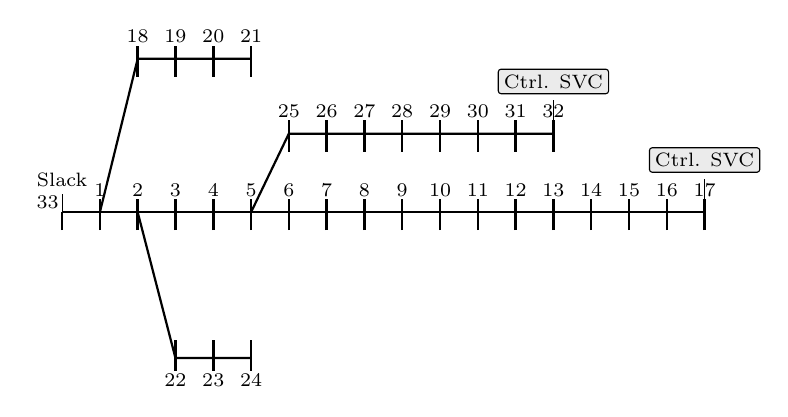
\begin{tikzpicture}[
        x=0.48cm,
        y=0.95cm,
        busbar/.style={line width=0.9pt},
        buslabel/.style={font=\scriptsize, inner sep=1pt, fill=white},
        svc/.style={draw, rounded corners=1pt, fill=black!8, inner sep=2pt, font=\scriptsize},
        feeder/.style={thick}
    ]
        % Slack bus and main feeder
        \coordinate (b33) at (0,0);
        \draw[busbar] ($(b33)+(0,-0.24)$) -- ($(b33)+(0,0.24)$);
        \node[buslabel, above left=0mm and 0mm of b33] {33};
        \node[above=2mm of b33, font=\scriptsize] {Slack};

        \foreach \n/\x in {1/1,2/2,3/3,4/4,5/5,6/6,7/7,8/8,9/9,10/10,11/11,12/12,13/13,14/14,15/15,16/16,17/17} {
            \coordinate (b\n) at (\x,0);
            \draw[busbar] ($(b\n)+(0,-0.24)$) -- ($(b\n)+(0,0.24)$);
            \node[buslabel, above=1.6mm of b\n] {\n};
        }

        % Upper laterals from buses 1 and 5
        \foreach \n/\x in {18/2,19/3,20/4,21/5} {
            \coordinate (b\n) at (\x,2.05);
            \draw[busbar] ($(b\n)+(0,-0.24)$) -- ($(b\n)+(0,0.24)$);
            \node[buslabel, above=1.6mm of b\n] {\n};
        }
        \foreach \n/\x in {25/6,26/7,27/8,28/9,29/10,30/11,31/12,32/13} {
            \coordinate (b\n) at (\x,1.05);
            \draw[busbar] ($(b\n)+(0,-0.24)$) -- ($(b\n)+(0,0.24)$);
            \node[buslabel, above=1.6mm of b\n] {\n};
        }

        % Lower lateral from bus 2
        \foreach \n/\x in {22/3,23/4,24/5} {
            \coordinate (b\n) at (\x,-1.95);
            \draw[busbar] ($(b\n)+(0,-0.24)$) -- ($(b\n)+(0,0.24)$);
            \node[buslabel, below=1.6mm of b\n] {\n};
        }

        % Feeder connections
        
        \draw[feeder] (b1) -- (b18) -- (b21);
        \draw[feeder] (b2) -- (b22) -- (b24);
        \draw[feeder] (b5) -- (b25) -- (b32);
        \draw[feeder] (b1) -- (b17);
        \draw[feeder] (b33) -- (b1);

        % Controlled SVC markers in shifted numbering
        \node[svc, above=5mm of b17] {Ctrl. SVC};
        \draw[thin] (b17) -- ++(0,0.45);
        \node[svc, above=5mm of b32] {Ctrl. SVC};
        \draw[thin] (b32) -- ++(0,0.45);
    \end{tikzpicture}%
    }
    \caption{Single-line diagram of the adopted IEEE 33-bus radial distribution system with the slack bus represented as bus 33 and the controlled FC--TCR compensators located at buses 17 and 32.}
    \label{fig:ieee33_singleline}
\end{figure}

\subsection{SVC Parameters}
\label{subsec:results_svc_parameters}

The electrical parameters and reactive-power operating ranges of the two
controlled compensators adopted in the 33-bus test system are summarized in
Table~\ref{tab:svc_parameters}.

\begin{table}[htbp]
\centering
\caption{Parameters of the static VAr compensators in the 33-bus test system}
\label{tab:svc_parameters}
\begin{threeparttable}
\footnotesize
\renewcommand{\arraystretch}{1.25}
\setlength{\tabcolsep}{3pt}
\begin{tabular}{@{}p{0.50\columnwidth}>{\centering\arraybackslash}p{0.20\columnwidth}>{\centering\arraybackslash}p{0.20\columnwidth}@{}}
\toprule
\textbf{Parameter} & \textbf{Bus 17} & \textbf{Bus 32} \\
\midrule
Bus number & 17 & 32 \\
Firing angles $\alpha_{j,\ell}$ (deg) & 90--180 & 90--180 \\
Control variables & $\alpha_{17,ab}$, $\alpha_{17,bc}$, $\alpha_{17,ca}$ & $\alpha_{32,ab}$, $\alpha_{32,bc}$, $\alpha_{32,ca}$ \\
\midrule
\multicolumn{3}{@{}l}{\textit{Thyristor-controlled reactor (TCR) --- per delta branch}} \\
\midrule
Inductance $L_j$ (mH) & 2.500 & 2.650 \\
Resistance $R_j$ ($\Omega$) & 0.001 & 0.001 \\
Reactance $X_{L,j}=\omega L_j$ ($\Omega$) & 0.942 & 0.999 \\
Reactance $X_{L,j}$ (pu)\tnote{a} & 0.00588 & 0.00623 \\
\midrule
\multicolumn{3}{@{}l}{\textit{Fixed capacitor bank (FC) --- per delta branch}} \\
\midrule
Capacitance $C_j$ ($\mu$F) & 2652.6 & 2652.6 \\
Reactance $X_{C,j}=1/\omega C_j$ ($\Omega$) & 1.000 & 1.000 \\
Reactance $X_{C,j}$ (pu)\tnote{a} & 0.00624 & 0.00624 \\
\midrule
\multicolumn{3}{@{}l}{\textit{Three-phase reactive-power range from harmonic power flow}} \\
\midrule
$Q_{\mathrm{SVC},j}^{\min}$ (kVAr)\tnote{b} & $-231.4$ & $-117.1$ \\
$Q_{\mathrm{SVC},j}^{\max}$ (kVAr)\tnote{c} & $+3210.8$ & $+3065.1$ \\
Control range $\Delta Q_{\mathrm{SVC},j}$ (kVAr) & $3442.2$ & $3182.2$ \\
\bottomrule
\end{tabular}

\begin{tablenotes}
\footnotesize
\item[a] Per-unit values on the system base: $S_b=1$ MVA, $V_b=12.66$ kV, and $Z_b=V_b^2/S_b=160.28\,\Omega$.
\item[b] $Q_{\mathrm{SVC},j}^{\min}$ corresponds to $\alpha_{j,\ell}=90^\circ$ in all delta branches, i.e., full TCR conduction; the negative sign indicates inductive operation.
\item[c] $Q_{\mathrm{SVC},j}^{\max}$ corresponds to $\alpha_{j,\ell}=180^\circ$ in all delta branches, i.e., complete blocking of the TCR branch; the positive sign indicates capacitive operation.
\end{tablenotes}
\end{threeparttable}
\end{table}

\noindent Therefore, the total installed compensation capacity of the two
controllable devices used in the optimization problem is

\begin{equation}
    S_{\mathrm{SVC,total}} \approx
    V_{\mathrm{LL,nom}}^2
    \sum_{j \in \{17,32\}} \sum_{\ell \in \{ab,bc,ca\}}
    \left|B_{\mathrm{SVC},j,\ell}\right|.
    \label{eq:svc_total_rating}
\end{equation}



\noindent For the adopted IEEE 33-bus distribution system,
$V_{\mathrm{LL,nom}} = 12.66$~kV. Equation~\eqref{eq:svc_total_rating} is
used to quantify the equivalent installed reactive-power capacity
associated with the controllable compensators, consistently with the
parameter set reported in Table~\ref{tab:svc_parameters}.

% -------------------------------------------------------------------------
\subsection{Balanced Loading Condition}
\label{subsec:balanced_results}
In this scenario, the three phases have identical active and reactive powers
at each load bus. It therefore verifies whether the branch-wise formulation
naturally recovers symmetrical SVC operation while satisfying the settings of
Section~\ref{subsec:numerical_settings}.

Fig.~\ref{fig:balanced_voltage_all_buses} presents the fundamental-frequency
voltage magnitude at all buses as a function of the common loading factor
$\lambda_k$. As expected for the radial feeder, the downstream buses are the
most sensitive to load growth and reach the lowest voltage magnitudes as
$\lambda_k$ increases. Nevertheless, the optimized SVC operation keeps the
voltages inside the adopted operating band over the feasible range identified
by the algorithm. Since the operating condition is balanced, the three phases
remain practically superimposed; therefore, a single set of overlapping
trajectories is observed for each bus.

\begin{figure}[!t]
    \centering
    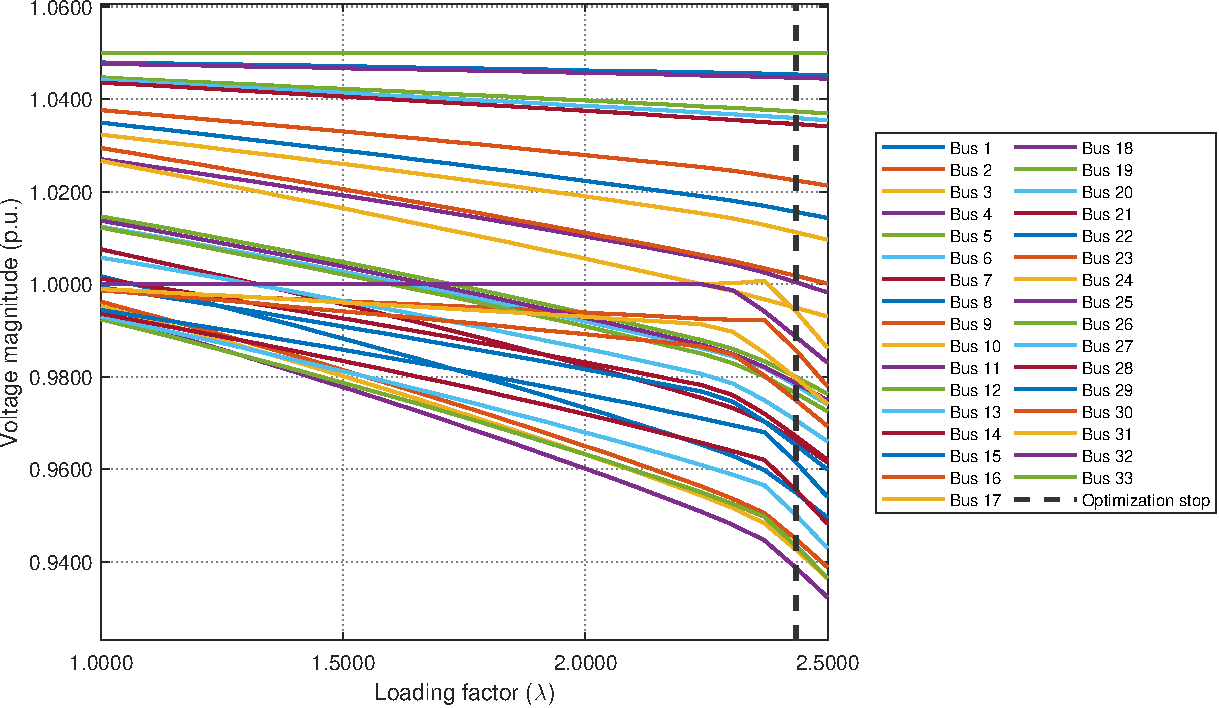
\includegraphics[width=\columnwidth]{caso equilibrado/figura_02.pdf}
    \caption{Voltage magnitude as a function of the loading factor for all
    buses in the balanced case with optimized SVC firing angles.}
    \label{fig:balanced_voltage_all_buses}
\end{figure}

The same voltage information is rearranged in
Fig.~\ref{fig:balanced_voltage_profiles}, which shows the feeder voltage
profile along the bus index for selected loading factors. This representation
highlights the spatial effect of load growth: the voltage drop becomes more
pronounced toward the end of the feeder, while the optimized compensators
support the controlled downstream regions and prevent the weakest buses from
leaving the admissible voltage range.

\begin{figure}[!t]
    \centering
    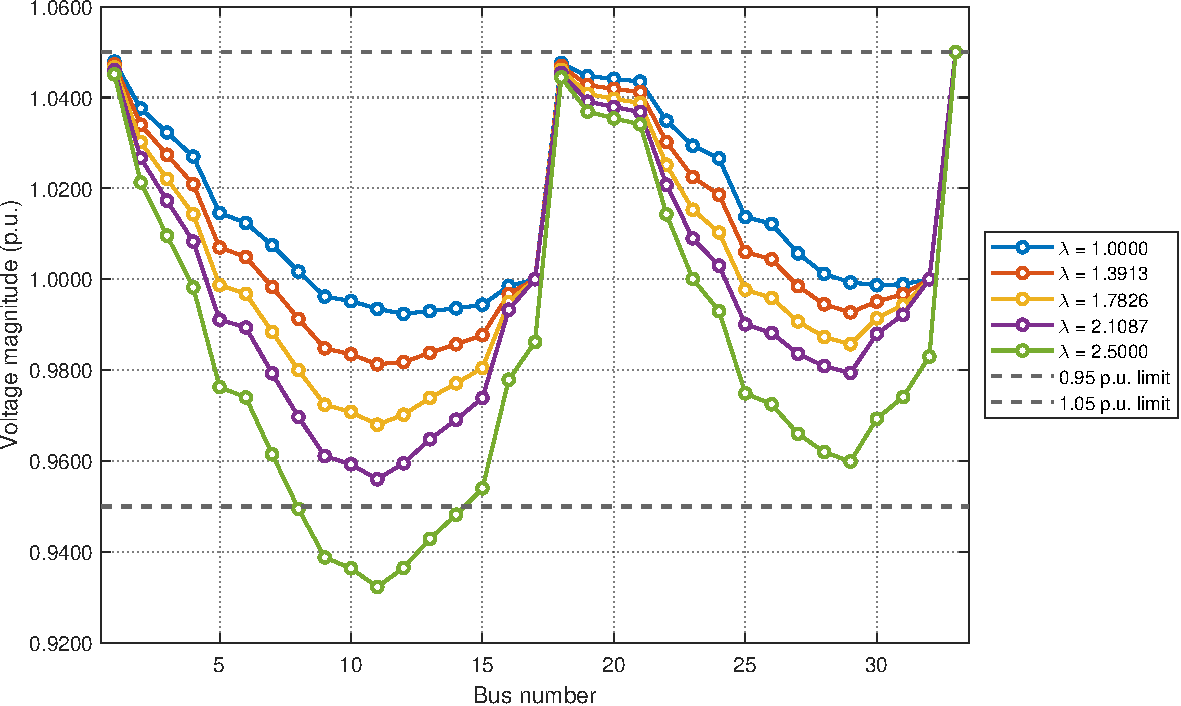
\includegraphics[width=\columnwidth]{caso equilibrado/figura_08.pdf}
    \caption{Voltage profiles of the balanced IEEE 33-bus system for
    different loading factors.}
    \label{fig:balanced_voltage_profiles}
\end{figure}

Figs.~\ref{fig:balanced_voltage_bus17} and
\ref{fig:balanced_voltage_bus32} isolate the controlled buses. Their three
phase trajectories overlap and remain within the prescribed limits throughout
the analyzed range.

\begin{figure}[!t]
    \centering
    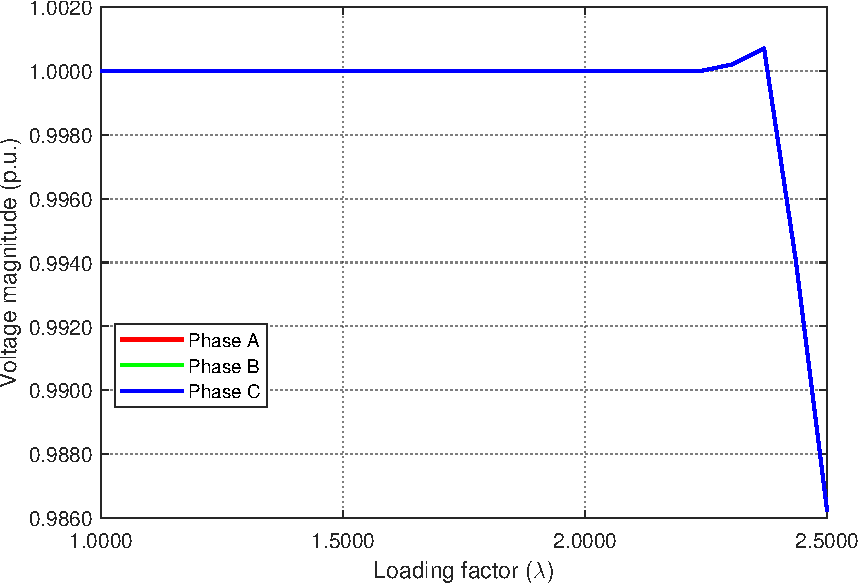
\includegraphics[width=\columnwidth]{caso equilibrado/figura_04.pdf}
    \caption{Voltage magnitude at the controlled SVC bus 17 as a function of
    the loading factor in the balanced case with optimized firing angles.}
    \label{fig:balanced_voltage_bus17}
\end{figure}

\begin{figure}[!t]
    \centering
    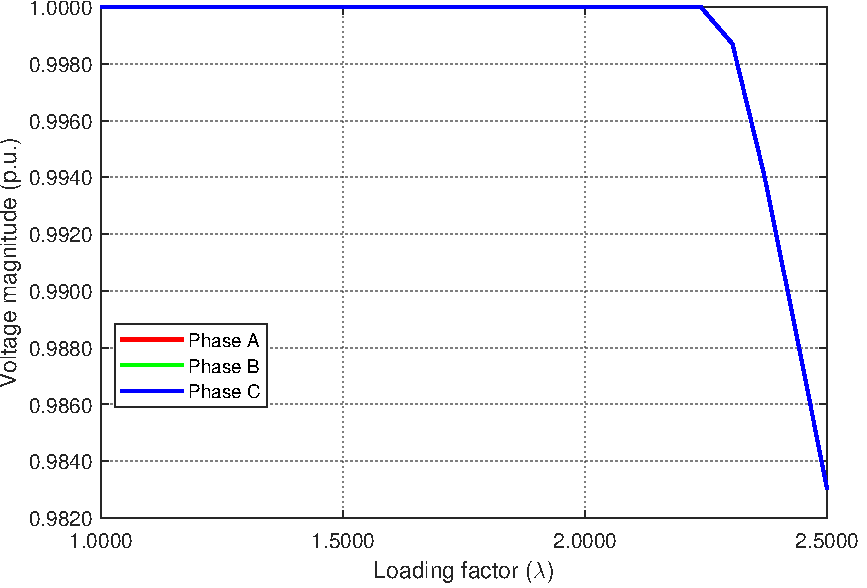
\includegraphics[width=\columnwidth]{caso equilibrado/figura_06.pdf}
    \caption{Voltage magnitude at the controlled SVC bus 32 as a function of
    the loading factor in the balanced case with optimized firing angles.}
    \label{fig:balanced_voltage_bus32}
\end{figure}

Fig.~\ref{fig:balanced_thdv_all_buses} summarizes the corresponding voltage
total harmonic distortion as a function of the common loading factor
$\lambda_k$. In this plot, each curve represents one bus of the feeder, while
the horizontal axis represents the progressive increase of the loading level.
The distortion remains below the adopted 8\% IEC compatibility level
throughout the simulated loading range, showing that the voltage-support
action obtained with the optimized FC--TCR compensators does not violate the
harmonic constraint. These comparatively low THD$_V$ values are consistent
with the balanced-delta cancellation property established in
\eqref{eq:triplen_delta_cancellation}. The THD$_V$ trajectories differ from bus
to bus because the harmonic voltages depend both on the non-triplen harmonic
currents injected by the controlled SVCs and on the harmonic impedance seen
from each bus.

\begin{figure}[!t]
    \centering
    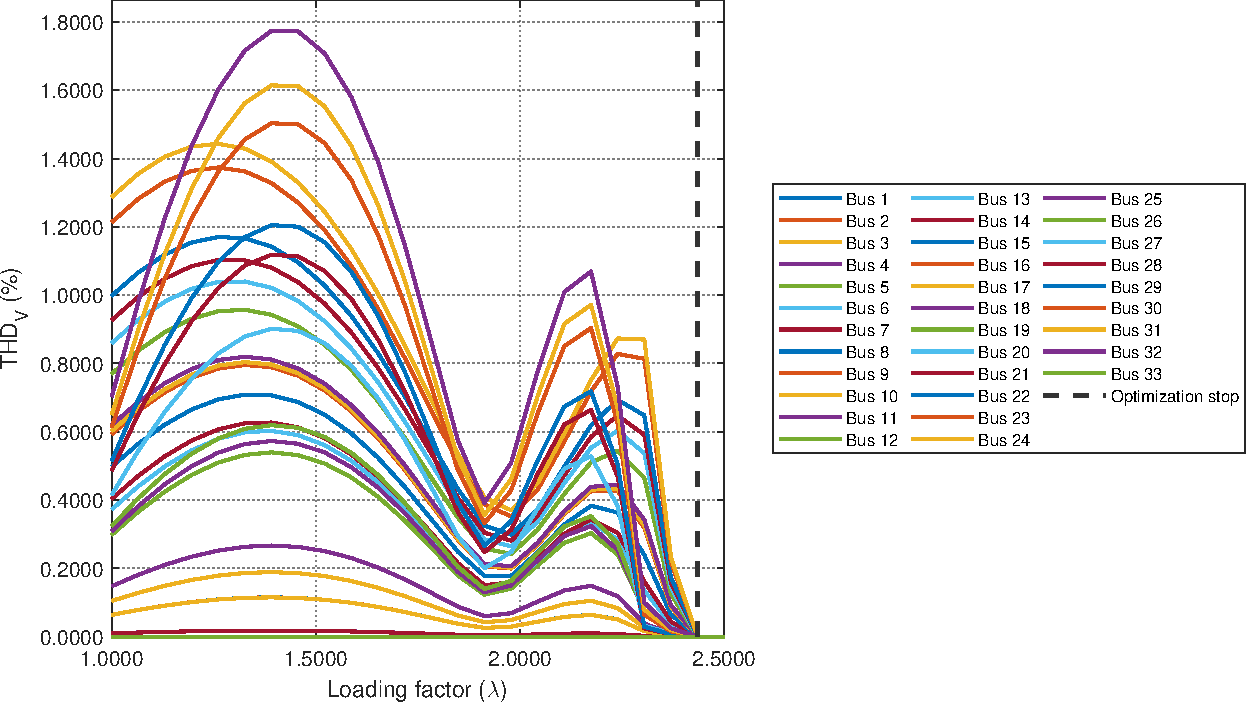
\includegraphics[width=\columnwidth]{caso equilibrado/figura_03.pdf}
    \caption{Voltage total harmonic distortion as a function of the loading
    factor for all buses in the balanced case.}
    \label{fig:balanced_thdv_all_buses}
\end{figure}

The controlled-bus detail in Figs.~\ref{fig:balanced_thdv_bus17} and
\ref{fig:balanced_thdv_bus32} likewise shows nearly coincident phase curves;
their local THD$_V$ values remain below the imposed limit.

\begin{figure}[!t]
    \centering
    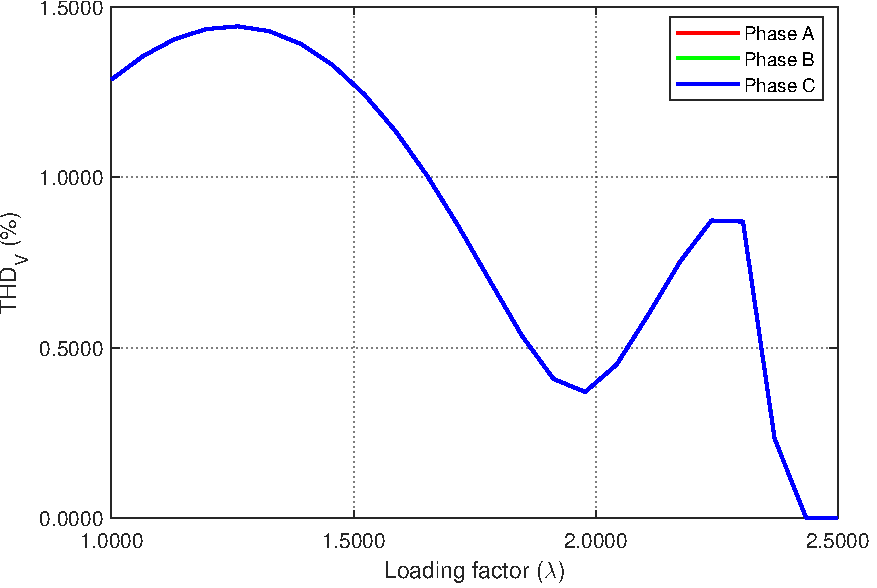
\includegraphics[width=\columnwidth]{caso equilibrado/figura_05.pdf}
    \caption{Voltage total harmonic distortion at bus 17 as a function of
    the loading factor in the balanced case.}
    \label{fig:balanced_thdv_bus17}
\end{figure}

\begin{figure}[!t]
    \centering
    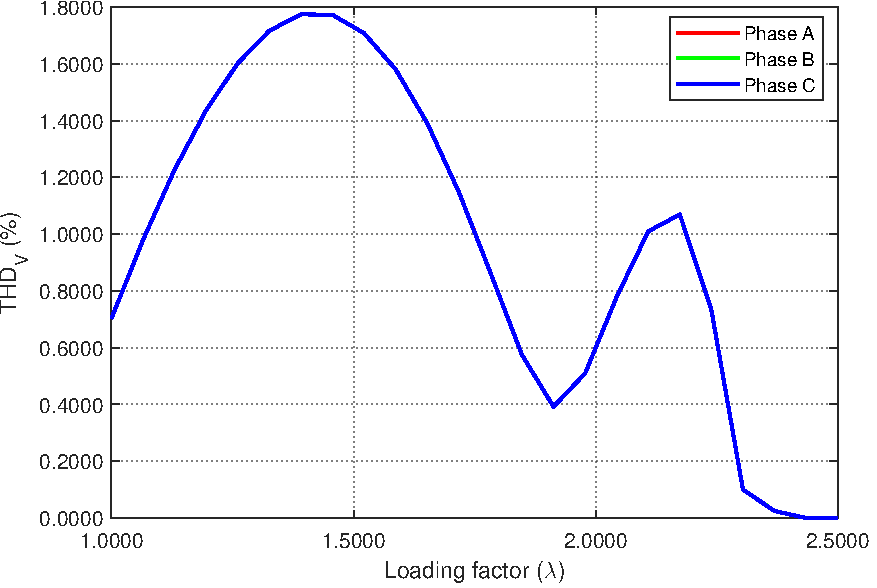
\includegraphics[width=\columnwidth]{caso equilibrado/figura_07.pdf}
    \caption{Voltage total harmonic distortion at bus 32 as a function of
    the loading factor in the balanced case.}
    \label{fig:balanced_thdv_bus32}
\end{figure}

Finally, Fig.~\ref{fig:balanced_firing_angles} shows the optimized firing
angles of the controlled SVCs. For low loading levels, the angles remain
close to $90^\circ$, corresponding to stronger TCR conduction. As the loading
factor increases, both firing angles move toward $180^\circ$, reducing the
reactor conduction interval and increasing the net capacitive effect of the
FC--TCR compensator. This behavior is physically consistent with the need for
additional voltage support under heavier loading conditions.

\begin{figure}[!t]
    \centering
    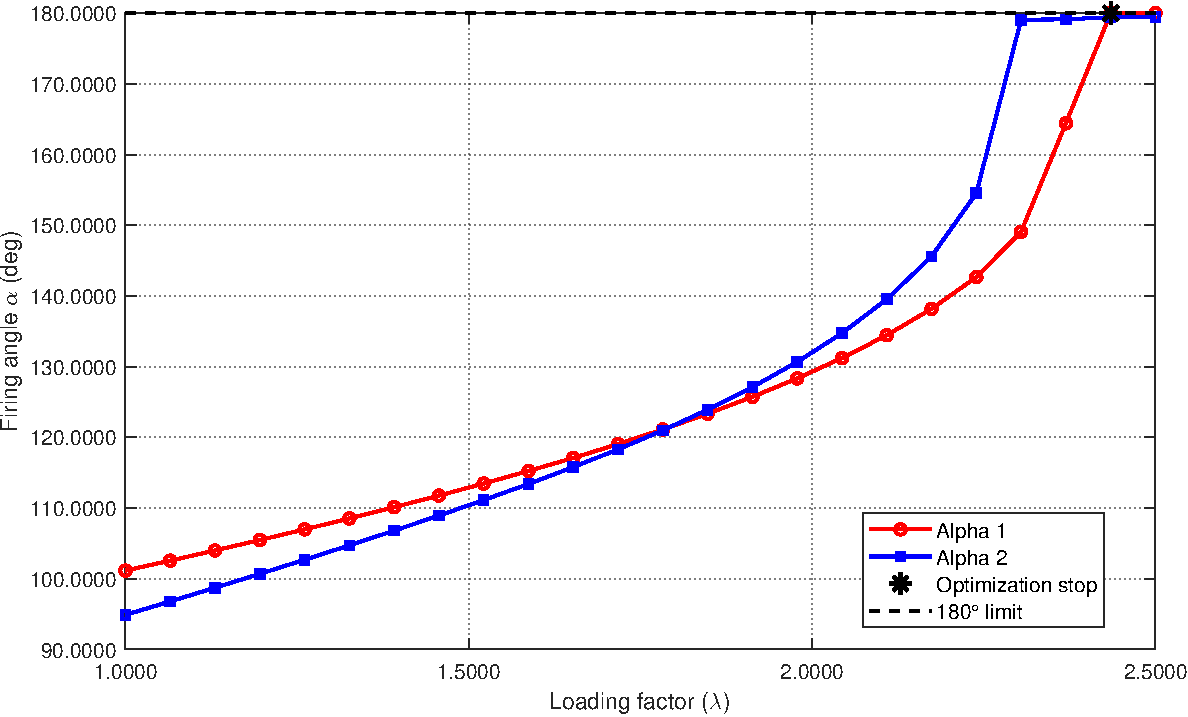
\includegraphics[width=\columnwidth]{caso equilibrado/figura_01.pdf}
    \caption{Optimized firing angles of the controlled SVCs as a function of
    the loading factor in the balanced case.}
    \label{fig:balanced_firing_angles}
\end{figure}

% -------------------------------------------------------------------------
\subsection{Three-Phase Unbalanced Loading Condition}
\label{subsec:unbalanced_results}

The unbalanced case uses the 24-hour, phase-dependent trajectory
$\boldsymbol{\Lambda}$ of~\eqref{eq:phase_load_curve}. The intentionally strict
limit $\mathrm{VUF}_{\max}=1\%$ tests active negative-sequence mitigation. No
external harmonic source is included, so the reported distortion results from
the two FC--TCR SVCs and the feeder harmonic response.

Fig.~\ref{fig:unbalanced_loading_profiles} shows the nonproportional phase
profiles. The same trajectory is applied at both controlled locations, so their
different responses arise from network conditions and control action rather
than from different imposed profiles.

\begin{figure}[!t]
    \centering
    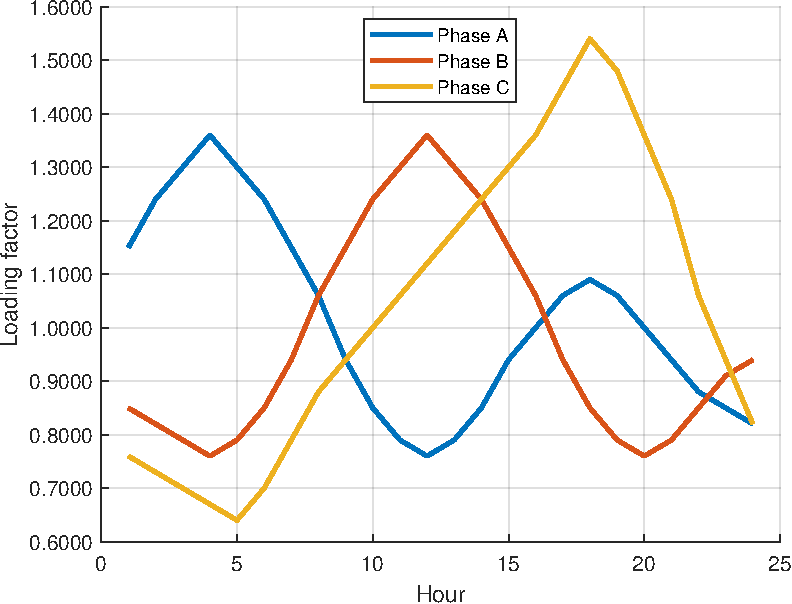
\includegraphics[width=\columnwidth]{caso desequilibrado/figura_01.pdf}
    \caption{Daily phase-dependent loading factors used in the unbalanced
    case.}
    \label{fig:unbalanced_loading_profiles}
\end{figure}

The main indicator of phase-balancing performance is the voltage unbalance
factor defined in~\eqref{eq:vuf}. Fig.~\ref{fig:unbalanced_vuf_bus17} compares
the VUF at bus 17 for the without-SVC and optimized-SVC cases. The case without SVC does not provide controllable reactive compensation for the
phase-dependent load variation, whereas the optimized controller uses the
independent delta-branch susceptances described in~\eqref{eq:svc_susceptance}
to keep the bus-17 VUF below the imposed 1\% limit. This confirms that the
negative-sequence term in the objective function and the explicit VUF
constraint in~\eqref{eq:optproblem} act together to enforce the desired
phase-balancing behavior.

\begin{figure}[!t]
    \centering
    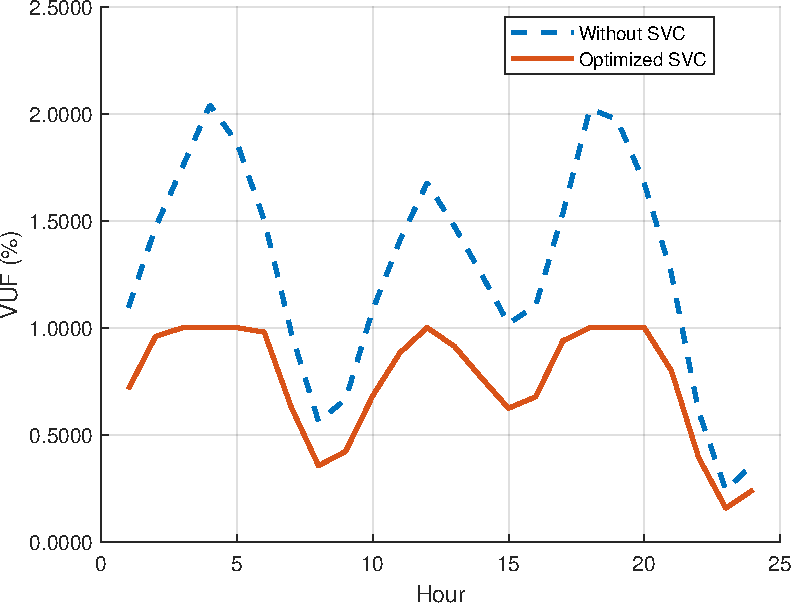
\includegraphics[width=\columnwidth]{caso desequilibrado/figura_02.pdf}
    \caption{Voltage unbalance factor at bus 17 in the unbalanced case without SVC and with
    optimized SVC operation.}
    \label{fig:unbalanced_vuf_bus17}
\end{figure}

Fig.~\ref{fig:unbalanced_v2_bus17} confirms that the VUF improvement is
associated with a reduction in the negative-sequence magnitude $|V_2|$, the
quantity penalized by~\eqref{eq:obj_neg}.

\begin{figure}[!t]
    \centering
    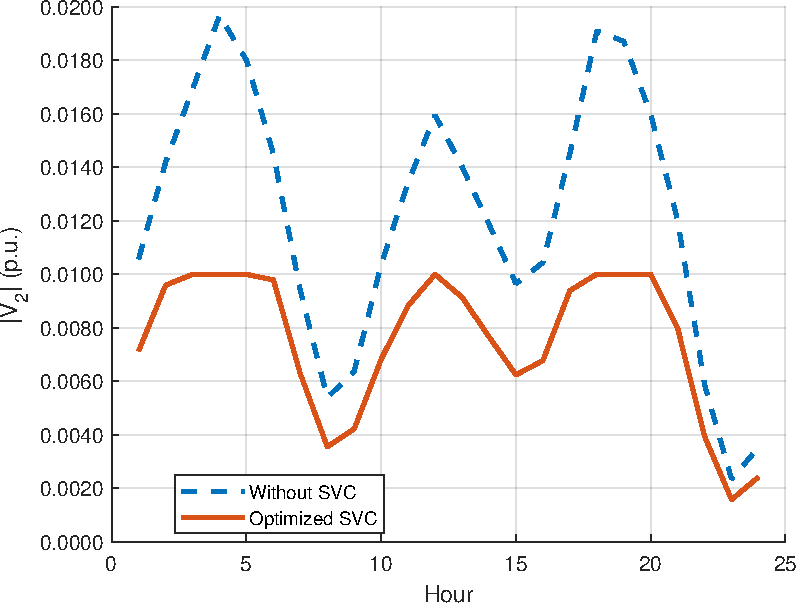
\includegraphics[width=\columnwidth]{caso desequilibrado/figura_03.pdf}
    \caption{Negative-sequence voltage magnitude at bus 17 in the unbalanced
    case.}
    \label{fig:unbalanced_v2_bus17}
\end{figure}

Fig.~\ref{fig:unbalanced_phase_voltage_bus17} presents the phase-voltage
magnitudes at bus 17 for the without-SVC and optimized-SVC cases. This figure links
the sequence-domain result to the phase-domain quantities used in the
phase-imbalance index. The optimized curves remain within the admissible
voltage range while reducing the separation among phases, which indicates that
the algorithm does not improve VUF by sacrificing voltage regulation.

\begin{figure}[!t]
    \centering
    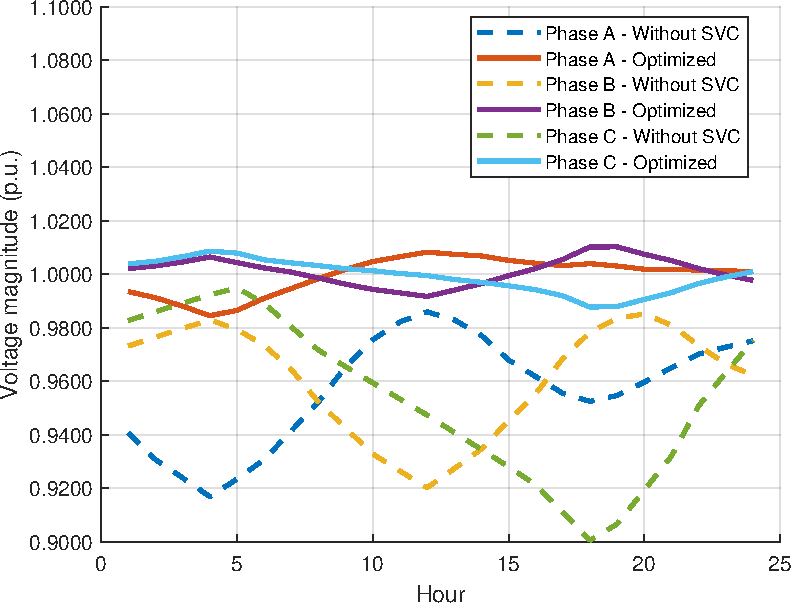
\includegraphics[width=\columnwidth]{caso desequilibrado/figura_04.pdf}
    \caption{Phase-voltage magnitudes at bus 17 in the unbalanced case without SVC and with
    optimized SVC operation.}
    \label{fig:unbalanced_phase_voltage_bus17}
\end{figure}

The control action responsible for these voltage and unbalance improvements is
shown in Fig.~\ref{fig:unbalanced_firing_angles_bus17}. In contrast with the
balanced case, the effective firing angles are not identical among phases.
Their separation indicates that the controller is redistributing the equivalent
reactive compensation among the delta branches, as allowed by the branch-wise
control variables of the proposed formulation. This behavior is the physical
mechanism that enables the SVC at bus 17 to supply compensation matched to the
phase-dependent operating condition.

\begin{figure}[!t]
    \centering
    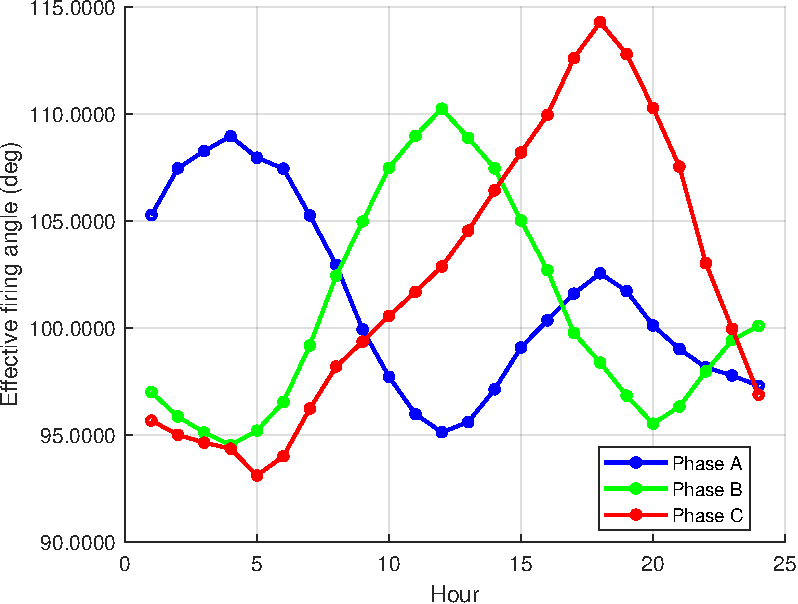
\includegraphics[width=\columnwidth]{caso desequilibrado/figura_05.pdf}
    \caption{Effective firing angles of the controlled SVC at bus 17 in the
    unbalanced case.}
    \label{fig:unbalanced_firing_angles_bus17}
\end{figure}

Fig.~\ref{fig:unbalanced_phase_voltage_deviation_bus17} reports the
phase-voltage deviations at bus 17. These curves are directly related to the
voltage-deviation component of the objective function. The optimized response
keeps the deviations closer to zero, showing that the controller simultaneously
tracks the voltage reference and reduces the phase-dependent dispersion caused
by the unbalanced daily load profile.

\begin{figure}[!t]
    \centering
    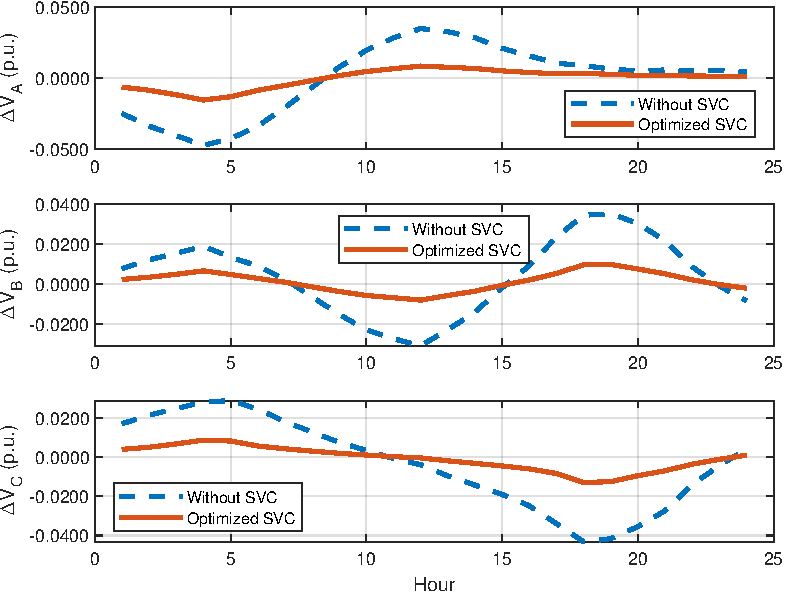
\includegraphics[width=\columnwidth]{caso desequilibrado/figura_07.pdf}
    \caption{Phase-voltage deviations at bus 17 in the unbalanced case without SVC and with
    optimized SVC operation.}
    \label{fig:unbalanced_phase_voltage_deviation_bus17}
\end{figure}

Fig.~\ref{fig:unbalanced_voltage_envelope_bus17} summarizes the voltage range
at bus 17 by means of maximum, minimum, and average values. This envelope
representation makes the phase dispersion easier to visualize than three
separate voltage traces. The optimized envelope is narrower and remains inside
the operating range, indicating that the proposed method improves voltage
support and phase balancing at the same controlled bus.

\begin{figure}[!t]
    \centering
    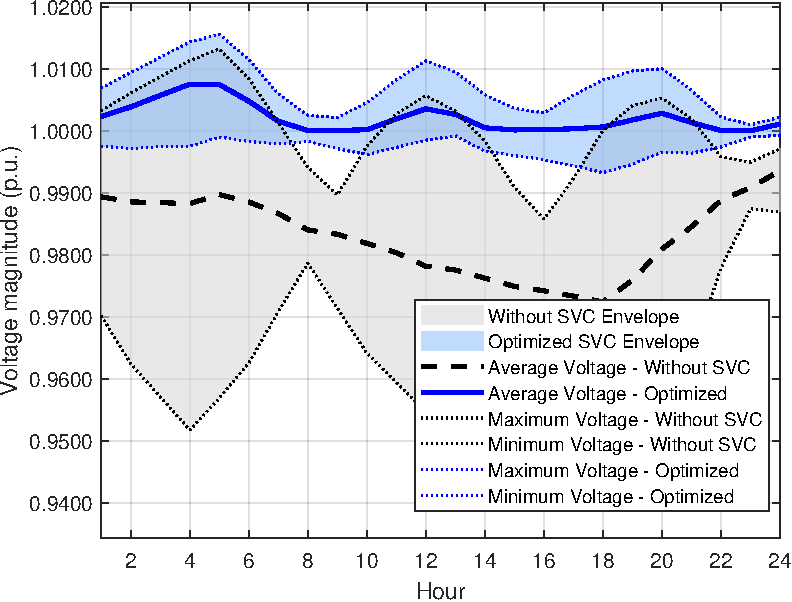
\includegraphics[width=\columnwidth]{caso desequilibrado/figura_09.pdf}
    \caption{Voltage envelope at bus 17 in the unbalanced case.}
    \label{fig:unbalanced_voltage_envelope_bus17}
\end{figure}

The harmonic impact of the branch-wise operation is assessed in
Fig.~\ref{fig:unbalanced_thdv_envelope_bus17}. Since no external harmonic
loads are present, the plotted THD$_V$ is produced by the harmonic current
injections of the two controlled FC--TCR devices and their interaction with the
network harmonic admittance. The optimized envelope remains below the adopted
8\% THD$_V$ limit, showing that the stricter VUF target at bus 17 is achieved
without violating the harmonic constraint in~\eqref{eq:optproblem}.

\begin{figure}[!t]
    \centering
    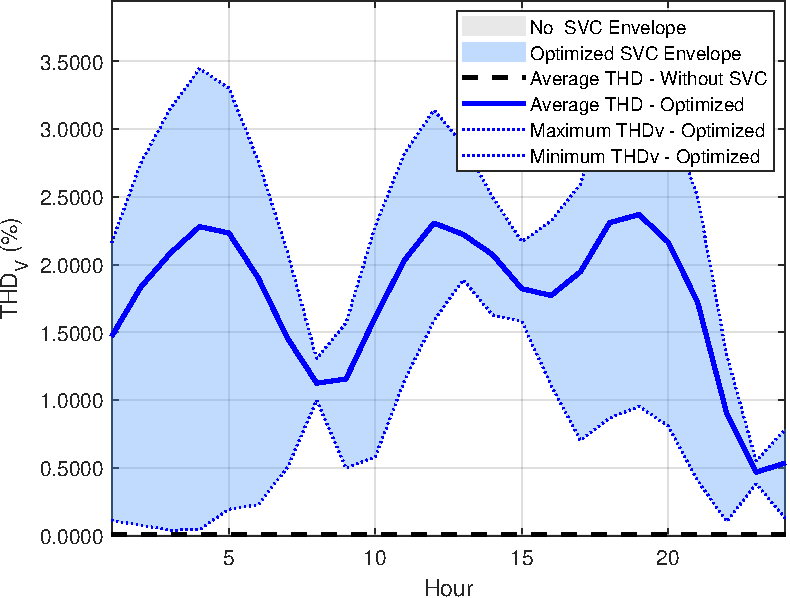
\includegraphics[width=\columnwidth]{caso desequilibrado/figura_10.pdf}
    \caption{Voltage total harmonic distortion envelope at bus 17 in the
    unbalanced case.}
    \label{fig:unbalanced_thdv_envelope_bus17}
\end{figure}

Fig.~\ref{fig:unbalanced_thdv_phase_bus17} details the optimized THD$_V$ by
phase at bus 17. The differences among phases are consistent with the
independent firing angles in Fig.~\ref{fig:unbalanced_firing_angles_bus17},
because each delta branch can generate a different harmonic-current spectrum.
Even with this asymmetric control action, the phase THD$_V$ values remain well
below the limit, confirming that the improvement in VUF is not obtained at the
expense of excessive harmonic distortion.

\begin{figure}[!t]
    \centering
    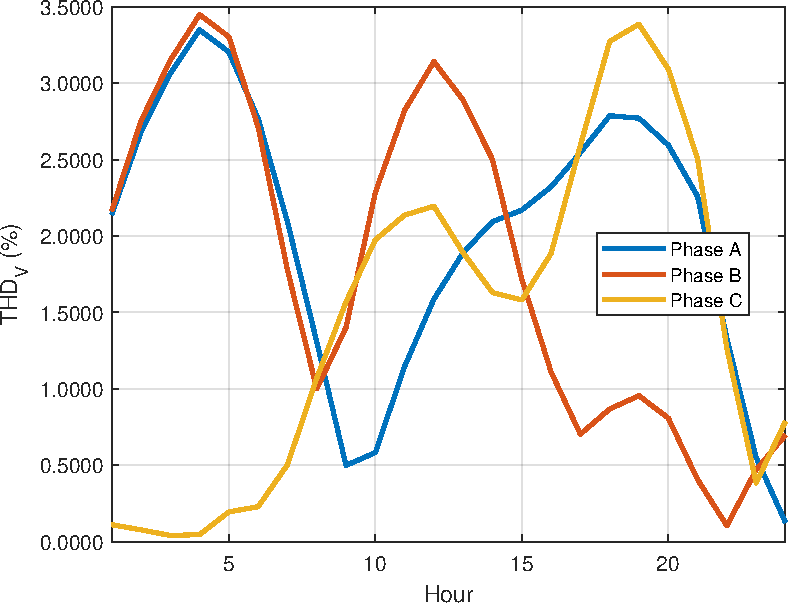
\includegraphics[width=\columnwidth]{caso desequilibrado/figura_11.pdf}
    \caption{Phase voltage total harmonic distortion at bus 17 in the
    optimized unbalanced case.}
    \label{fig:unbalanced_thdv_phase_bus17}
\end{figure}


For bus 32, only VUF, negative-sequence voltage, branch firing angles, voltage
envelope, and THD$_V$ envelope are shown, because their interpretation follows
the definitions already discussed for bus 17.

Fig.~\ref{fig:unbalanced_vuf_bus32} shows that optimized branch-wise control
also keeps the bus-32 VUF below 1\%.

\begin{figure}[!t]
    \centering
    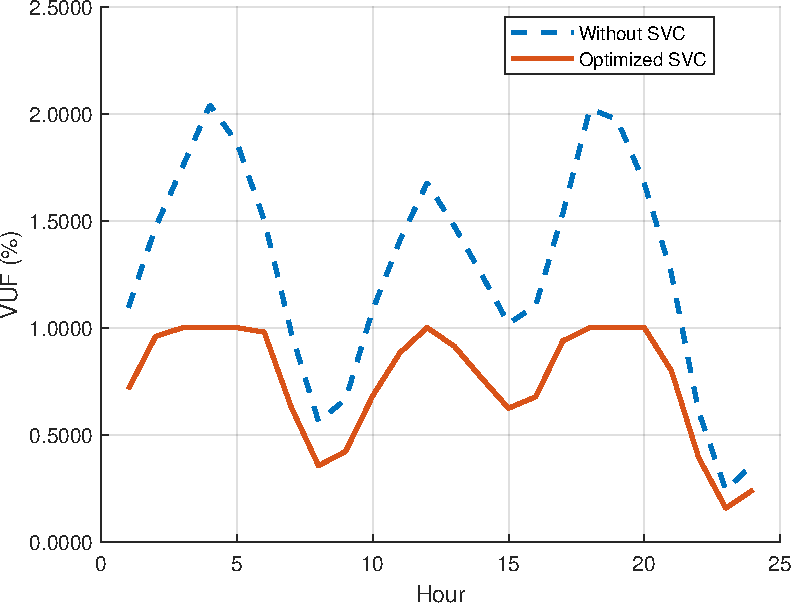
\includegraphics[width=\columnwidth]{caso desequilibrado/barra 32/figura_11.pdf}
    \caption{Voltage unbalance factor at bus 32 in the unbalanced case without
    SVC and with optimized SVC operation.}
    \label{fig:unbalanced_vuf_bus32}
\end{figure}

The corresponding reduction in $|V_2|$ is shown in
Fig.~\ref{fig:unbalanced_v2_bus32}.

\begin{figure}[!t]
    \centering
    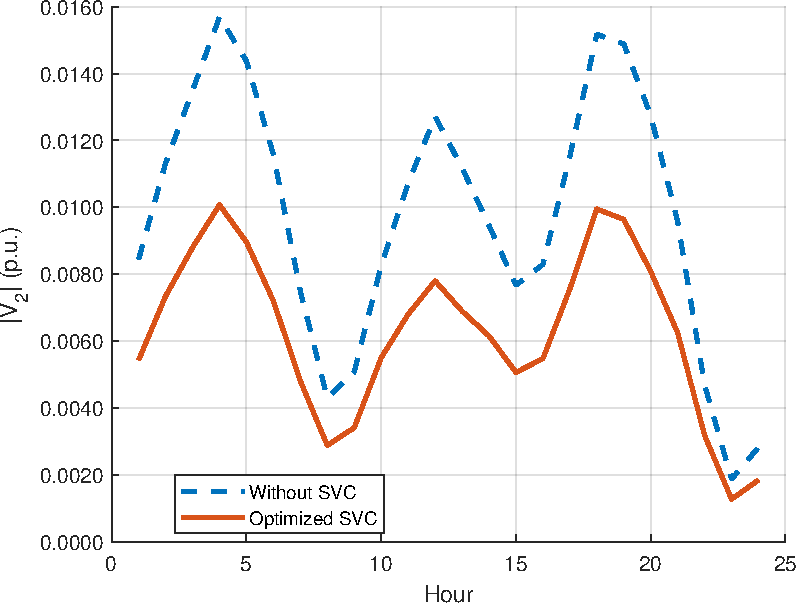
\includegraphics[width=\columnwidth]{caso desequilibrado/barra 32/figura_10.pdf}
    \caption{Negative-sequence voltage magnitude at bus 32 in the unbalanced
    case.}
    \label{fig:unbalanced_v2_bus32}
\end{figure}

The control variables selected by the optimizer for bus 32 are shown in
Fig.~\ref{fig:unbalanced_firing_angles_bus32}. The phase-dependent firing-angle
trajectories indicate that the compensator is not operated as a balanced
three-phase reactive source; instead, the delta branches are adjusted
independently to provide the asymmetric compensation required by the unbalanced
load trajectory.

\begin{figure}[!t]
    \centering
    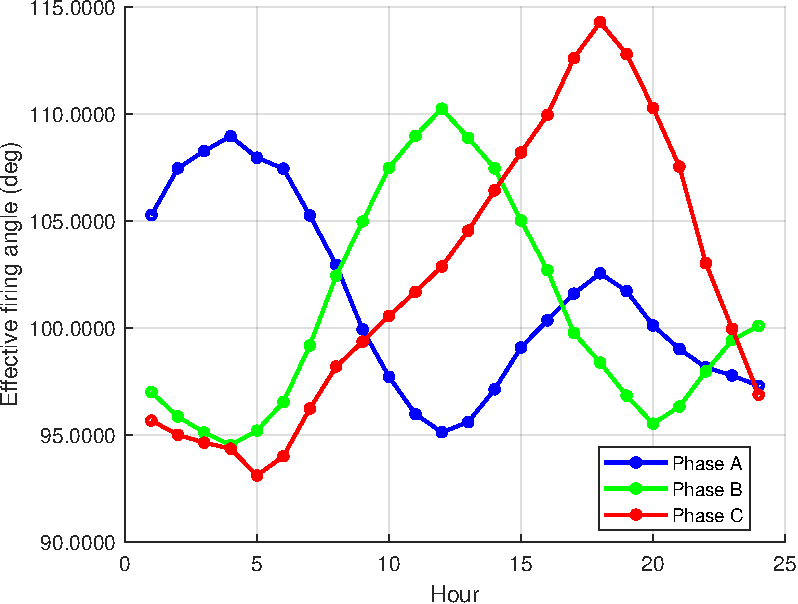
\includegraphics[width=\columnwidth]{caso desequilibrado/barra 32/figura_08.pdf}
    \caption{Effective firing angles of the controlled SVC at bus 32 in the
    unbalanced case.}
    \label{fig:unbalanced_firing_angles_bus32}
\end{figure}

Fig.~\ref{fig:unbalanced_voltage_envelope_bus32} summarizes the voltage
magnitudes at bus 32 through the minimum, maximum, and average phase-voltage
envelopes. The optimized envelope verifies that the VUF reduction is obtained
while preserving the voltage profile within the admissible operating range.

\begin{figure}[!t]
    \centering
    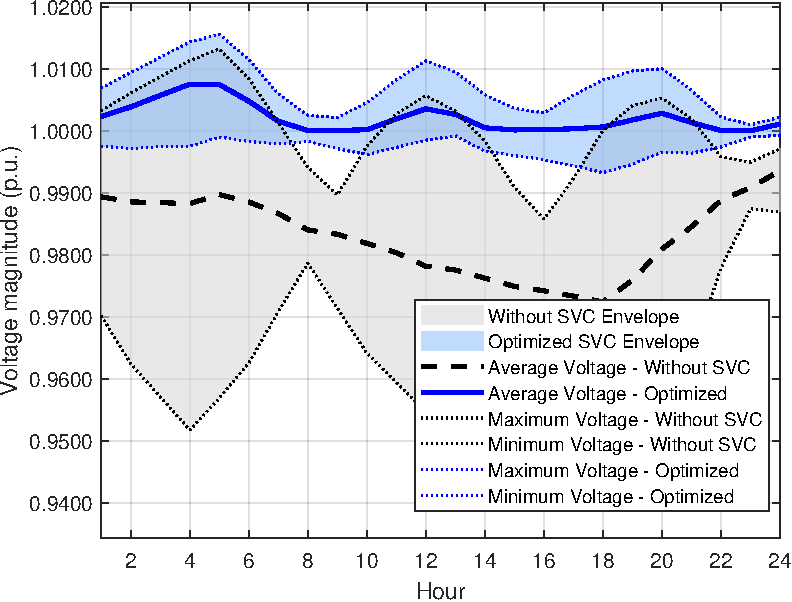
\includegraphics[width=\columnwidth]{caso desequilibrado/barra 32/figura_04.pdf}
    \caption{Voltage envelope at bus 32 in the unbalanced case.}
    \label{fig:unbalanced_voltage_envelope_bus32}
\end{figure}

Finally, the THD$_V$ envelope in
Fig.~\ref{fig:unbalanced_thdv_envelope_bus32} remains below 8\%.

\begin{figure}[!t]
    \centering
    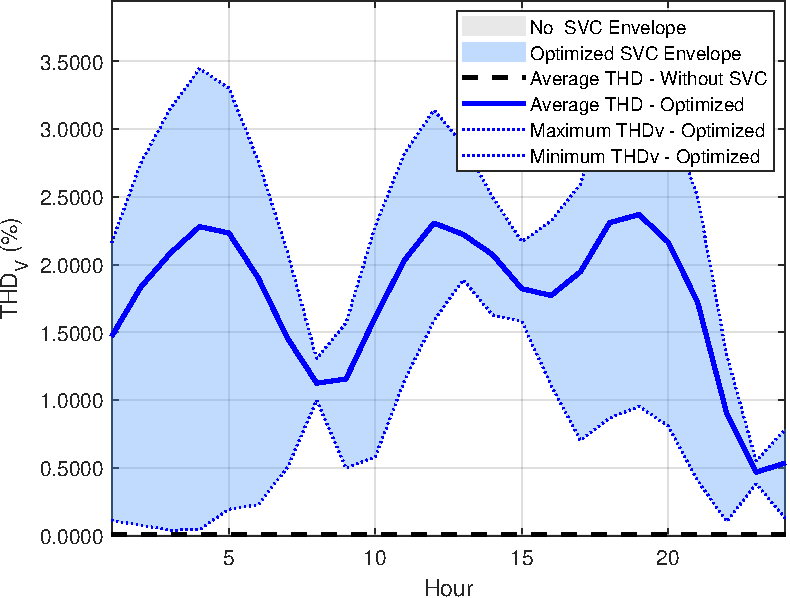
\includegraphics[width=\columnwidth]{caso desequilibrado/barra 32/figura_03.pdf}
    \caption{Voltage total harmonic distortion envelope at bus 32 in the
    unbalanced case.}
    \label{fig:unbalanced_thdv_envelope_bus32}
\end{figure}

Table~\ref{tab:unbalanced_performance_summary} consolidates the two-bus
comparison. At buses 17 and 32, optimized control reaches the 1\% VUF target,
raises the minimum voltage from 0.9005 to 0.9845~pu and from 0.9393 to
0.9933~pu, respectively, and reduces the maximum phase spread. THD$_V$
increases because the SVCs are the nonlinear sources in this case, but remains
below 8\%.

\begin{table}[!t]
\centering
\caption{Summary of the unbalanced-case performance}
\label{tab:unbalanced_performance_summary}
\setlength{\tabcolsep}{4pt}
\renewcommand{\arraystretch}{1.08}
\begin{tabular}{@{}lcc@{}}
\toprule
Case & Bus 17 & Bus 32 \\
\midrule
Max. VUF, no SVC (\%) & 2.0405 & 1.5876 \\
Max. VUF, opt. SVC (\%) & 1.0000 & 1.0000 \\
Max. $|V_2|$, no SVC (pu) & 0.0197 & 0.0157 \\
Max. $|V_2|$, opt. SVC (pu) & 0.0100 & 0.0101 \\
Min. $V$, no SVC (pu) & 0.9005 & 0.9393 \\
Min. $V$, opt. SVC (pu) & 0.9845 & 0.9933 \\
Max. spread, no SVC (pu) & 0.0778 & 0.0607 \\
Max. spread, opt. SVC (pu) & 0.0241 & 0.0168 \\
Max. THD$_V$, no SVC (\%) & 0.0091 & 0.0100 \\
Max. THD$_V$, opt. SVC (\%) & 5.3047 & 3.4477 \\
VUF limit, no SVC & No & Yes \\
VUF limit, opt. SVC & Yes & Yes \\
THD$_V$ limit, no SVC & Yes & Yes \\
THD$_V$ limit, opt. SVC & Yes & Yes \\
\bottomrule
\end{tabular}
\end{table}

\section{Conclusion}
\label{sec:conclusion}

This paper proposed a nonlinear optimization methodology for controlling
SVCs in three-phase distribution systems. The formulation integrates MICTH
with a generic device current-injection interface and a constrained optimization
layer, so its scope is not inherently limited to the connection or internal
arrangement selected for the case study. The numerical implementation uses
delta-connected FC--TCR compensators and a branch-wise firing-angle strategy,
allowing the $ab$, $bc$, and $ca$ branches to be adjusted independently. This
implementation extends the role of the SVC beyond conventional balanced
reactive-power support, permitting phase-dependent compensation while explicitly
enforcing voltage, THD, and voltage-unbalance constraints.

The simulations performed on the IEEE 33-bus test system confirmed that the
proposed controller improves the voltage profile and increases the loading
capability of the controlled buses without exceeding the prescribed power-quality
limits. Under balanced loading, the optimized firing angles remain nearly equal
among phases, indicating that the formulation naturally reproduces the expected
behavior of a conventional three-phase compensator. Under unbalanced loading,
however, the independent branch control of the selected delta implementation
provides additional flexibility,
reducing negative-sequence voltage components and phase-magnitude dispersion
while maintaining THD$_V$ within the adopted compatibility threshold.

The main contribution of the work is therefore the integration of voltage
support, harmonic-performance assessment, and phase-balancing objectives into a
single constrained optimization framework for SVC operation. The results
also emphasize that harmonic constraints should not be treated as secondary
checks after voltage regulation has been achieved. Because thyristor-controlled
compensators may alter the harmonic operating point of the feeder, voltage
support and harmonic distortion must be considered simultaneously during the
control process.

Although the results are promising, the present study is limited to a benchmark
feeder and steady-state operating scenarios. Future work should extend the
methodology to larger and more detailed distribution networks, time-series
simulations, distributed generation, electric-vehicle charging, and uncertainty
in load and measurement data. Additional research should also address faster
optimization routines, alternative SVC connections and internal arrangements,
coordination with other Volt/Var resources, and experimental validation using
hardware-in-the-loop or real-time digital simulation platforms.


\bibliographystyle{IEEEtran}
\bibliography{references}

\clearpage
\appendices
\section{System Data Used in the Simulations}
\label{app:system_data}

This appendix summarizes the active data set used to build the 33-bus test
system in the harmonic power-flow simulations. The notation is kept consistent
with the formulation adopted in the paper: $i$ denotes a bus, $\phi\in\Phi$
denotes a phase, $h$ denotes a harmonic order, and $j$ denotes an SVC bus. The
base quantities are $V_b=12.66$~kV, $S_b=1$~MVA, and
$Z_b=V_b^2/S_b=160.28~\Omega$. The fundamental frequency is 60~Hz, and the
harmonic set is $\mathcal{H}=\{1,3,5,7,11,13\}$. Bus 33 is the slack bus,
with balanced voltage magnitude 1.05~pu and phase angles $0^\circ$,
$-120^\circ$, and $120^\circ$.

The line parameters in Table~\ref{tab:appendix_line_data} are the per-phase
series resistance and reactance before per-unit conversion. In the three-phase
model, the same self impedance is assigned to phases $a$, $b$, and $c$. The
mutual phase-coupling terms used in the data file are generated from the
corresponding self terms as one eighth of the self resistance and inductance,
and the shunt capacitance terms are derived from those mutual inductance
entries.

\begin{table}[H]
\centering
\caption{Line data of the adopted 33-bus feeder}
\label{tab:appendix_line_data}
\setlength{\tabcolsep}{3pt}
\renewcommand{\arraystretch}{1.0}
\begin{tabular}{@{}lcc@{}}
\toprule
Branch & $R$ ($\Omega$) & $X$ ($\Omega$) \\
\midrule
33--1 & 0.0922 & 0.047 \\
1--2 & 0.493 & 0.2511 \\
2--3 & 0.366 & 0.1864 \\
3--4 & 0.3811 & 0.1941 \\
4--5 & 0.819 & 0.707 \\
5--6 & 0.1872 & 0.6188 \\
6--7 & 0.7114 & 0.2351 \\
7--8 & 1.03 & 0.74 \\
8--9 & 1.044 & 0.74 \\
9--10 & 0.1966 & 0.065 \\
10--11 & 0.3744 & 0.1238 \\
11--12 & 1.468 & 1.155 \\
12--13 & 0.5416 & 0.7129 \\
13--14 & 0.591 & 0.526 \\
14--15 & 0.7463 & 0.545 \\
15--16 & 1.299 & 1.721 \\
16--17 & 0.732 & 0.574 \\
1--18 & 0.164 & 0.1565 \\
18--19 & 1.5042 & 1.3554 \\
19--20 & 0.4095 & 0.4784 \\
20--21 & 0.7089 & 0.9373 \\
2--22 & 0.4512 & 0.3083 \\
22--23 & 0.898 & 0.7091 \\
23--24 & 0.896 & 0.7011 \\
5--25 & 0.203 & 0.1034 \\
25--26 & 0.2842 & 0.1447 \\
26--27 & 1.059 & 0.9337 \\
27--28 & 0.8042 & 0.7006 \\
28--29 & 0.5075 & 0.2585 \\
29--30 & 0.9744 & 0.963 \\
30--31 & 0.3105 & 0.3619 \\
31--32 & 0.341 & 0.5302 \\
\bottomrule
\end{tabular}
\end{table}

The phase-dependent load values used at each operating point are obtained from
Table~\ref{tab:appendix_load_data} according to
\eqref{eq:phase_load_scaling}. Entries written as a subtraction, such as
$90-200$, indicate that a fixed distributed-generation contribution is
subtracted from the local demand at that bus. In the uploaded data file, the
phase scaling coefficients are implemented through $A=1000\,d_a/S_b$,
$B=1000\,d_b/S_b$, and $C=1000\,d_c/S_b$, where $d_a$, $d_b$, and $d_c$ are
the phase loading multipliers. The ZIP composition is set as a constant-power
model, i.e., $P_{\mathrm{p}}=Q_{\mathrm{p}}=1$ and
$P_{\mathrm{i}}=P_{\mathrm{z}}=Q_{\mathrm{i}}=Q_{\mathrm{z}}=0$.

\begin{table}[H]
\centering
\caption{Nominal phase-load coefficients used in the ZIP load block}
\label{tab:appendix_load_data}
\setlength{\tabcolsep}{3pt}
\renewcommand{\arraystretch}{1.0}
\begin{tabular}{@{}ccc@{}}
\toprule
Bus & $P_i^0$ (kW) & $Q_i^0$ (kVAr) \\
\midrule
1 & 100 & 60 \\
2 & 90 & 40 \\
3 & 120 & 80 \\
4 & 60 & 30 \\
5 & 60 & 20 \\
6 & 200 & 100 \\
7 & 200 & 100 \\
8 & 60 & 20 \\
9 & 60 & 20 \\
10 & 45 & 30 \\
11 & 400 & 350 \\
12 & 60 & 35 \\
13 & 120 & 80 \\
14 & 60 & 10 \\
15 & 60 & 20 \\
16 & 60 & 20 \\
17 & 70 & 20 \\
18 & $90-200$ & 40 \\
19 & 90 & 40 \\
20 & 90 & 40 \\
21 & 90 & 40 \\
22 & $190-200$ & 50 \\
23 & 420 & 200 \\
24 & 420 & 200 \\
25 & $60-200$ & 25 \\
26 & 60 & 25 \\
27 & 60 & 20 \\
28 & 120 & 70 \\
29 & 200 & 600 \\
30 & 150 & 70 \\
31 & 210 & 100 \\
32 & $60-200$ & 40 \\
\bottomrule
\end{tabular}
\end{table}

The transformer data in Table~\ref{tab:appendix_transformer_data} define the
series impedances and connection codes used in the feeder model. The SVC
entries in Table~\ref{tab:appendix_svc_data} correspond to the two controllable
compensators used by the optimizer. Their conduction windows are implemented as
$T_{\mathrm{on},1}=\alpha_j$, $T_{\mathrm{off},1}=270^\circ-(\alpha_j-90^\circ)$,
$T_{\mathrm{on},2}=\alpha_j$, and
$T_{\mathrm{off},2}=450^\circ-(\alpha_j-90^\circ)$.

\begin{table}[H]
\centering
\caption{Transformer data used in the test feeder}
\label{tab:appendix_transformer_data}
\setlength{\tabcolsep}{3pt}
\renewcommand{\arraystretch}{1.0}
\begin{tabular}{@{}ccccc@{}}
\toprule
No. & From--to & Conn. & $R_{tr}$ & $X_{tr}$ \\
\midrule
1 & 7--8 & 11 & 0.01 & 0.17615 \\
2 & 4--9 & 11 & 0.01 & 0.55618 \\
3 & 7--9 & 11 & 0.01 & 0.11001 \\
4 & 4--7 & 11 & 0.01 & 0.20912 \\
5 & 5--6 & 11 & 0.01 & 0.25201 \\
\bottomrule
\end{tabular}
\end{table}

\begin{table}[H]
\centering
\caption{Active FC--TCR SVC entries in the simulation data file}
\label{tab:appendix_svc_data}
\setlength{\tabcolsep}{3pt}
\renewcommand{\arraystretch}{1.0}
\begin{tabular}{@{}ccccc@{}}
\toprule
Bus $j$ & Conn. & $L_j$ & $R_j$ & $C_j$ \\
\midrule
17 & Delta & 2.50 & 0.001 & 2652.60 \\
32 & Delta & 2.65 & 0.001 & 2652.60 \\
\bottomrule
\end{tabular}
\end{table}

\end{document}
